\documentclass[letterpaper,conference]{IEEEtran}
%\pdfoutput=0 % force latex (not pdflatex) -- to be able to include .eps images
% (automated conversion is disabled for arxiv)

%\usepackage{epsfig}

\usepackage{setspace}

%\usepackage[dvipdfmx]{graphicx}
\usepackage{graphicx}
%\usepackage{epstopdf}

%\usepackage{subfigure}
\usepackage{calc}
%\usepackage{amssymb}
%\usepackage{amstext}
%\usepackage{amsmath}
%\usepackage{amsthm}
\usepackage{multicol}
%\usepackage{pslatex}
\usepackage{apalike}
%\usepackage{SCITEPRESS}     % Please add other packages that you may need BEFORE the SCITEPRESS.sty package.
\usepackage{url}
\usepackage[ruled,linesnumbered]{algorithm2e}
\usepackage{color}
\usepackage{caption}

\usepackage{multirow}

%\subfigtopskip=0pt
%\subfigcapskip=0pt
%\subfigbottomskip=0pt

% \doublespacing
\begin{document}

% \newfloat{listing}
% \floatname{listing}{Listing}


% i.e. don't!
%\hyphenation{TOTAL\_DELAY}
\hyphenation{HarmonicIO} 

%Apache Spark and HarmonicIO: a Benchmark Comparison for Feature Extraction from High-Throughput Data Streams 

%Apache Spark Streaming and HarmonicIO: a Benchmark Comparison for High-Throughput Feature Extraction

%\title{Apache Spark Streaming and HarmonicIO: a Benchmark Comparison for High-Throughput Microscopy Image Feature Extraction}
%\title{Apache Spark Streaming, Kafka and HarmonicIO: A~Performance and Architecture Comparison for Streaming Applications in Enterprise and Scientific Computing Domains}
\title{Apache Spark Streaming, Kafka and HarmonicIO: A~Performance Benchmark and Architecture Comparison for Enterprise and Scientific Computing}

\author{
\IEEEauthorblockN{
Ben Blamey\IEEEauthorrefmark{1}, Andreas Hellander\IEEEauthorrefmark{1} and Salman Toor\IEEEauthorrefmark{1}
}
\IEEEauthorblockA{
\IEEEauthorrefmark{1} Department of Information Technology, Division of Scientific Computing, Uppsala University, Sweden\\ 
Email: \{Ben.Blamey, Andreas.Hellander, Salman.Toor\}@it.uu.se 
}
}

\maketitle
% force page numbers for 'bench' submission
\thispagestyle{plain}
\pagestyle{plain}

%%%%%%%%%%%%%%%%%%%%%%%%%%%%%%%%%%%%%%%%%%%%%%%%%%%%%%%%%%%%%%%%%%%%%%%%%%%%%%%%
\begin{abstract}
%This paper introduces the HASTE SCaaS (scientific computing as a service) platform, a general scientific computing platform for stream processing, with a focus on spatial-temporal and time-series data, and a novel interestingness-based tiered storage platform. The first use case for the platform is presented, a pipeline for the online analysis of a stream of microscopy images. Focusing the characteristics of this use case, performance 

%%Studies have demonstrated that Apache Spark, Flink and related frameworks can perform stream processing at very high frequencies,
% have been shown to perform message stream processing very well.
%%whilst tending to focus on small messages with a computationally light `map' stage for each message; a common enterprise use case. 
%Motivated by an interest in stream processing in the context of typical scientific computing applications, 
%%We add to these benchmarks by broadening the domain to include loads with larger messages (leading to network-bound throughput), and that are computationally intensive (leading to CPU-bound throughput) in the map phase; in order to evaluate applicability of these frameworks to scientific computing applications.
%, such as high-throughput microscopy, and other applications sharing their characteristics.
%{\color{red}{AH: shorten this and move details to Introduction}}
%%We present a performance benchmark comparison between Apache Spark Streaming (ASS) under both file and TCP streaming modes; and HarmonicIO, comparing maximum throughput over a broad domain of message sizes and CPU loads.
%%We find that relative performance varies considerably across this domain, with the chosen means of stream source integration having a big impact.
%, and that consequently, high performance does not always generalize over the whole domain, and discuss this in relation to theoretical bounds, and the underlying architectures -- together with a feature comparison.
%With a focus on network-bound cases, consequently network topology and especially P2P architectures for stream processing are discussed.
%Looking wholistically at the scientific computing context, 
%We explore broader issues related to the scientific computing use case, such as ease of adoption (incl. deployment, configuration) by a scientists and others without specialist knowledge of these frameworks.
%%We offer recommendations for choosing and configuring the frameworks, 
%present a simple approach to measuring maximum throughput, 
%%and present a benchmarking toolset developed for this study.
%discuss challenges in measuring maximum throughput 


% This paper presents a benchmark of stream processing throughput comparing Apache Spark Streaming (under file-, TCP socket- and Kafka-based stream integration), with a prototype P2P stream processing framework, \emph{HarmonicIO}.
% Maximum throughput for a spectrum of stream processing loads are measured, specifically, those with large message sizes (up to 10MB), and heavy CPU loads -- more typical of scientific computing use cases (such as microscopy), than enterprise contexts.
% A detailed exploration of the performance characteristics with these streaming sources, under varying loads, reveals an interplay of performance trade-offs, uncovering the boundaries of good performance for each framework and streaming source integration. We compare with theoretic bounds in each case.
% Based on these results, we suggest which frameworks and streaming sources are likely to offer good performance for a given load.
% Broadly, the advantages of Spark's rich feature set comes at a cost of sensitivity to message size in particular -- common stream source integrations can perform poorly in the 1MB-10MB range.
% The simplicity of HarmonicIO offers more robust performance in this region, especially for raw CPU utilization.

Many scientific computing applications generate streams where message size can exceed one megabyte, in contrast with smaller message sizes in enterprise contexts (order kilobytes, often XML or JSON). Furthermore, the processing cost of messages in scientific computing applications are usually an order of magnitude higher than in typical enterprise applications. Frameworks such as Apache Spark offer high throughput processing of streams -- with such ‘enterprise’ characteristics, as well as scalability, with high resilience and many other desirable features.   Motivated by the development of near real-time image processing pipelines for roboticized microscopy, we evaluate the suitability of Apache Spark for streams more typical of scientific computing applications, those with large message sizes (up to 10MB), and heavy per-message CPU load, under typical stream integrations. For comparison, we benchmark a P2P stream processing framework, \emph{HarmonicIO}, developed in-house. Our study reveals a complex interplay of performance trade-offs, revealing the boundaries of good performance for each framework and integration over a wide domain of application loads. Based on these results, we suggest which are likely to offer good performance for a given load. Broadly, the advantages of Spark's rich features makes its performance sensitive to message size in particular, whereas the simplicity of HarmonicIO offers more robust performance, and better CPU utilization.



% In conclusion, many scientific computing, or otherwise unorthodox streaming use cases could benefit from the multitude of features offered by frameworks such as Apache Spark 




%which can be broadly characterized by small message size (typically ~1KB), computationally light map operations, which an emphasis on sorting opera


%, albeit for particular use cases (small messages), 

%We discuss the architectures of both frameworks, their suitability to different stream processing problems - investigating the performance state-of-the-art-stream processing frameworks for image analysis tasks.
\end{abstract}
%%%%%%%%%%%%%%%%%%%%%%%%%%%%%%%%%%%%%%%%%%%%%%%%%%%%%%%%%%%%%%%%%%%%%%%%%%%%%%%%
%\onecolumn \maketitle \normalsize \vfill
%\textcolor{green}{ST: Options for the title: 
% \\
% - Apache Spark and HarmonicIO: a Benchmark Comparison for Feature Extraction from High-Throughput Data Streams 
% \\
% - Apache Spark Streaming and HarmonicIO: a Benchmark Comparison for High-Throughput Feature Extraction
% }

% %\textcolor{blue}{BB:no mention of SCaaS vision in paper}
% %\textcolor{blue}{BB:findings, contribs, diff vs. other bench studies}
% %\textcolor{blue}{BB: DIDN'T LOOK AT multiple-sources -- P2P IS BEST THING ABOUT HarmonicIO -- another paper?}
% %\textcolor{blue}{BB: LITTLE FOCUS ON MICROSCOPY - its a CPU cost, and a message size. Pipeline was actually benchmarked in the previous study.}

% %\textcolor{blue}{BB: one could argue that the emphasis (atleast obstensibly) on microscopy limits the audience scope (and hence impact), if I saw ‘microscopy’ in the title I might think this was a ‘systems’ paper and skip to the next paper (if I wasn’t involved in microscopy)
% What we actually have is a broad exploration of performance (from a HPC viewpoint - CPU+network bounds) of a popular framework, highlighting some deficiencies (outside of its intended use case), and showcasing a framework which is actually more robust. Thats much broader than microscopy.}

\begin{IEEEkeywords}Stream Processing; Apache Spark, HarmonicIO, high-throughput microscopy; HPC; Benchmark; XaaS.\end{IEEEkeywords} % HASTE

\section{Introduction}\label{intro}

%\textcolor{blue}{page limit = 1.5 (including Title, Authors information, Abstract and Introduction)}

%\textcolor{blue}{ Rationale / Key contributions / Summarize other sections }

%\textcolor{blue}{How might we do online stream processing? There are lots of frameworks for stream processing}

Several stream processing frameworks have gained wide adoption over the last decade or so.
%(Apache Flink~\cite{carboneApacheFlinkStream2015}, Apache Spark Streaming~\cite{zahariaApacheSparkUnified2016}, Flume~\cite{apacheflumeApacheFlume2016}); suitable for high-volume, high-reliability stream processing workloads. Their development has been motivated by analysis of data from cloud, web and mobile applications. 
%For example, 
Apache Flume is designed for the analysis of server application logs. Apache Spark improves upon the Apache Hadoop framework~\cite{ApacheHadoop2011} for distributed computing, and was later extended with streaming support~\cite{zahariaApacheSparkUnified2016}. Apache Flink~\cite{carboneApacheFlinkStream2015} was later developed primarily for stream processing.
% (in Flink, batching is handled as a special case of streaming, whilst in Spark the opposite is true). 

%\textcolor{blue}{their features look attractive!}

%There are some very popular, high quality frameworks for distributed stream processing (of small messages) their features:
These frameworks boast 
excellent performance, scalability, data security, processing guarantees, and efficient, parallelized computation; together with high-level stream processing APIs (augmenting familiar map/reduce with stream-specific functionality such as windowing). These features are attractive for scientific computing -- including imaging applications in the life-sciences, and simulation output more generally.


%Apache Spark in particular...
%Apache Spark was originally developed for batch operations, with a focus on in-memory caching of intermediate results to improve on the performance of Hadoop, where data is typically written to a distributed file system and read at each stage. Spark facilitates a more interactive user experience, allowing more ad-hoc analysis, something which was difficult with Hadoop. This smart caching behavior is combined with functionality to track the lineage of the calculations, to support deterministic re-calculation in the event of errors and node failure, together with a host of other features, built around the Resilient Distributed Dataset (RDD)~\cite{Zaharia:2012:RDD:2228298.2228301}. 
%The core RDD Spark API ~\cite{Zaharia:2012:RDD:2228298.2228301} allows for distributed computation, whilst recording the provenance and derivation of data between calculations, thus allowing for deterministic re-computation in cases of error and node failure, with a high level API that makes such details transparent to the application developer. 


Previous studies have shown that these frameworks are capable of processing message streams on the order of 1 million or more messages per second, but focus on enterprise use cases with textual rather than binary content, and of message size perhaps a few KB. Additionally, the computational cost of processing an individual message may be relatively small (e.g. parsing JSON, and applying some business logic). By contrast, in scientific computing domains messages can be much larger (order of several MB, in medical imaging and systems biology applications~\cite{blameyAdaptingSecretaryHiring2019}). In other scientific computing applications, message sizes can be smaller \cite{CharacterizationDOEMiniapps}.

Due to the different design priorities for streaming frameworks, a single benchmark will not be adequate to cover various features. However, an alternative approach is to use a standard use case to compare different frameworks. The presented study highlights the needs of scientific communities, importance of streaming frameworks for scientific workloads and the difference in the inherent nature of the scientific datasets as compared to the enterprise context.

We selected Apache Spark for this study because of its popularity, and to allow comparison to earlier studies. Its core \emph{RDD} API~\cite{Zaharia:2012:RDD:2228298.2228301} allows for deterministic re-computation in cases of error and node failure, various high-level APIs which make such details transparent to the application developer. Apache Spark can scale successfully to 1000s of nodes~\cite{xinApacheSparkFastest2014}. Spark Streaming was a later addition, leveraging the batch functionality for a streaming context by creating a new batch every few seconds (the batch interval). As with batch operations, data is further subdivided into partitions for distribution and scheduling. The newer \emph{Direct DStream} integration approach is used with Kafka in this study. 
%The Streaming API augments map/reduce operators (familiar from a batch processing context) with new functionality specifically for streams, such as windowing. 

%Stream processing pipelines are built from these operators, and the frameworks themselves manage the processing parallelization and data transfer -- with various guarantees in relation to fault handling. 
%These features, and the maturity of the frameworks themselves, together with the extent of their support community is attractive for our microscopy use case, and indeed scientific computing applications more widely.





%\textcolor{blue}{challenges adopting these in a scientific computing context? typical setup -- lots of tiny JSON documents:}


%querying an ML model).

%\textcolor{blue}{ we want to do online processing of an image stream for our microscopy application}

Our motivating use case 
is the development of a cloud pipeline for the processing of streams of microscopy images. Existing systems for working with such datasets have largely focused on offline processing: our online processing (processing the `live' stream), 
is relatively novel for the image microscopy domain. %, with a growing interest in automation in that sector (citation?).
%Indeed, adoption of such frameworks in IoT contexts is growing rapidly. 
%\textcolor{blue}{ whats the challenge?}
Electron microscopes generate high-frequency streams of large, high-resolution image files (message sizes 1-10MB), and feature extraction is computationally intensive. This is typical of many scientific computing use cases: where files have binary content, 
with execution time dominated by the per-message `map' stage. Our pipeline consists of a single `map' operator. 
%analysis of each unit might be independent (i.e. map only) -- well-suited to parallel processing at large scale.
%Files can be of any size, but in an online streaming context,
%Limiting ourselves to streaming (rather than batch) processing, we might consider file sizes not exceeding 10MB or so.%\footnote{~This equates to the order of 1 sec transfer over a 1GB/s connection.}
Thereby, we investigate how well the performance of enterprise stream processing frameworks (such as Apache Spark) translates to loads more characteristic of scientific computing, for example, microscopy image stream processing, by benchmarking under a spectrum of conditions representative of both. We do this by varying both the processing cost of the map stage, and the message size to expand on previous studies.
%, and by extension similar workloads in a scientific context. 
%In particular, we investigate how well typical configurations of these frameworks perform when processing streams of messages with sizes on the order of megabytes, and/or with larger per-message CPU cost -- contrasting with the focus in previous benchmarking studies on small messages and lighter map stages.

%We undertook performance benchmarking of Apache Spark Streaming (ASS), in various configurations, varying the message size and the computational cost of processing each message -- simulating a wide spectrum of use cases, expanding on previous studies.
%, which have focused on particular use cases: small message sizes, and small message processing costs -- this paper investigates how the performance of Spark with such applications extends to other use cases -- particularly network-bound use cases -- and indeed how frameworks with other architectures and implementation compare. 

For comparison, we measured the performance of HarmonicIO~\cite{torruangwatthanaHarmonicIOScalableData2018a} -- a research prototype with a which has a P2P-based architecture, under the same conditions. 
% we're simulating stream processing applications, with tunable CPU load, and tunable message size.
%{\color{green}{Two main contributions:}}
This paper contributes:

\begin{itemize}
\item A performance comparison of an enterprise grade framework (Apache Spark) for stream processing to a streaming framework tailored for scientific use cases (HarmonicIO).

\item An analysis of these results, and comparison with theoretical bounds -- relating the findings to the architectures of the framework when integrated with various streaming sources. We find that performance varies considerably according to the application loads -- quantifying where these transitions occur.
%whilst this is unsurprising, our study quantifies such transition points.

\item Benchmarking tools for Apache Spark Streaming, %able to determine maximum throughput for file and TCP streaming, 
with tunable message size and CPU load per message -- to explore this domain as a continuum.
%allowing us to explore performance characteristics over a broad range of use cases, both `enterprise message processing' use cases similar to previous studies, and more scientific use cases.

\item Recommendations for choosing frameworks and their integration with stream sources, especially for atypical stream processing applications, highlighting some 
 limitations of both frameworks especially for scientific computing use cases.  %, and the microscopy image use case in particular; and discussion of challenges and techniques for benchmarking.
 
\end{itemize}

% Whilst the microscopy use case motivates an interest in 'medium sized' files, in a online stream processing context, we don't tend to work with enormous files anyway, because we're limited to the hardware. (and, files vs. file partitions becomes an argument about semantics).

%%\textcolor{blue}{round up with signposting?}

\section{BACKGROUND: STREAM PROCESSING OF IMAGES IN THE HASTE PROJECT}\label{background}

% Our main motivation for considering streaming applications where messages are relatively large binary objects (BLOBs) and where each processing task can be quite CPU intensive comes from work on smart cloud systems for prioritizing and organizing data from 
% high-throughput ~\cite{wollmanHighThroughputMicroscopy2007}, and high-content imaging (HCI) experiments in which highly automated experimental setups are used to screen molecular libraries and assess the effects of compounds on cells using microscopy imaging. 

High-throughput ~\cite{wollmanHighThroughputMicroscopy2007}, and high-content imaging (HCI) experiments are highly automated experimental setups which are used to screen molecular libraries and assess the effects of compounds on cells using microscopy imaging. Work on smart cloud systems for prioritizing and organizing data from these experiments is our motivation for considering streaming applications where messages are relatively large binary objects (BLOBs) and where each processing task can be quite CPU intensive.

% BLIND
In the HASTE project\footnote{\texttt{http://haste.reserach.it.uu.se}} -- a collaboration between Uppsala University, Stockholm University, Vironova AB and AstraZeneca, we are investigating methodology for near real-time filtering and control of image streams from such HCI platforms. 


%Microscopy image analysis is a research domain of its own (especially within biosciences, and many other disciplines), with a huge variety of image analysis techniques employed for different image resolutions and applications (tissues, cells, etc.), and an extensive history of software tools and frameworks exist to assist and automate such analysis (see \cite{schindelinFijiOpenSource2012} for an overview). Yet, the approach is generally \emph{offline} -- analyzing batches of images after they have been collected.
%With high throughput microscopy (HTM)~\cite{wollmanHighThroughputMicroscopy2007} techniques, often involving robotic automation, image streams can be generated over several hours or days; generating many images requiring analysis.
%\textcolor{blue}{ why do we want to do online str proc? interestingness, haste}
%Online processing of microscopy images allows 
%By contrast, 
Our goal of \emph{online} analysis of the microscopy image stream allows both the quality of the images to analyzed (highlighting any issues with the equipment, sample preparation, etc.) as well as detection of characteristics (and changes) in the sample itself \emph{during the experiment}. 
%This has a number of benefits, which, generalizing the dual notion of image quality to one of abstract `interestingness', apply to a broad class of scientific experiments:
%which can be generalized a much broader class o both concepts to other experiments as `interestingness' 
%(1) it creates opportunities for automated (or semi-automated) real time control of microscopy and other scientific equipment, as part of a wider goal of increasing automation in bioscience laboratories; online analysis facilitates decision-making about the `interestingness' of an image, or set of images, (2) which can be considered when making a choice about where (and indeed if) to store the associated data -- less interesting or garbage data can be discarded or stored in cheaper, lower performance storage. (3) such measures of interestingness can also be used to decide whether to perform further computational processing of images -- similarly, (4) the most interesting data can be selectively presented to scientists and technicians for review and to facilitate decision making during an experiment. For example, microscopes could record some samples more closely. Overall, given this interestingness measure, we can prioritize available storage, compute, and indeed human resources on the data most important to overarching research goals. 
%%\textcolor{blue}{what is SC use case}
%Characterizing the scientific computing use is difficult given the breadth of applications, but
%perhaps these properties 
%A recent masters thesis characterized potential streaming rates for a production HCI platform at one of the industry collaborators in the [BLIND] %HASTE project, and found that current setups would be able to produce 38 frames/second with image sizes on the order of 10Mb \cite{lugnegaard2018building}. Clearly, such image streams have different characteristics than many enterprise stream analytics applications. In particular: % -- online analysis of this image stream is novel.
%A recent masters thesis characterized potential streaming rates for a production HCI platform at one of the industry collaborators in the [BLIND] %HASTE project, and found that 
Industry setups for high-content imaging can produce 38 frames/second with image sizes on the order of 10MB \cite{lugnegaard2018building}. 
These image streams, like other scientific use cases, have different characteristics than many enterprise stream analytics applications: % -- online analysis of this image stream is novel.

%The characteristics of scientific data streams generally differ from many typical enterprise applications:

\begin{itemize}
\item Messages are binary (not textual, JSON, XML, etc.).
\item Messages are larger (order MBs, not bytes or KBs).
\item The initial map phase can be computationally expensive, and perhaps dominate execution time.
\end{itemize}



Our goal is to create a general pipeline able to process streams with these characteristics (and image streams in particular).
%with an emphasis on spatial-temporal analysis. Our SCaaS -- \emph{Scientific Computing as a Service} platform will to allow domain scientists to work with large datasets in an economically efficient way
%, through the use of hierarchical storage, for example, 
%without needing to manage infrastructure and software themselves. 
Apache Spark Streaming (ASS) has many of the features needed to build such a platform, with rich APIs suitable for scientific applications, and proven performance for small messages with computationally light map tasks. However, it is not clear how well this performance translates to the regimes of interest to the HASTE project. This paper explores the performance of ASS for a wide range of application characteristics, and compares it to a research prototype streaming framework HarmonicIO. %; developed within the [BLIND] project. 

%HASTE wil use the domain-specific interestingness functions (in the case of microscopy, image quality, and observed phenomena) to decouple decisions about storage and further processing from the scientific application itself, and the infrastructure used -- i.e. given a user-specified application and suitable interestingness measure, our SCaaS infrastructure can intelligently determine the allocation of compute and hierarchical storage resources, and selecting data for subsequent processing, without the user being concerned with details of available infrastructure. We hope to allow users to specify high-level trade-offs between economic cost, and storage/compute -- and leave the framework to reconcile this policy with the application and infrastructure. 

%Furthermore, we hope to offer SCaaS -- \emph{Scientific Computing as a Service} with HASTE; to allow scientists to work with large datasets in an economically efficient way, through the use of hierarchical storage, for example, without needing to manage infrastructure and software themselves.
%Development of a cloud streaming platform suitable for scientific datasets, and their applications -- 
%This paper explores the suitability of stream processing frameworks, and compares their performance relating it to architecture and features, in the first step towards this goal.
% hierarchical COMPUTE not just hierarchical storage

\section{EXISTING BENCHMARKING STUDIES}\label{benchmarking}
%\textcolor{blue}{ on benchmarking (frameworks themselves are discussed earlier)}
%\textcolor{blue}{ Short survey of stream processing, and in particular benchmarking performance comparison stream processing for images / image analysis pipelines.
%... existing work on benchmarking stream processing frameworks?}
% %\textcolor{green}{ ST: We can move this section either right after the introduction (section-II) so readers will get an overview before going into deep-down details. Otherwise, we can push it before conclusion for the sack of completeness. As section-III it comes somewhat in the middle. }
%\textcolor{green}{ ST: For this section we can use the text available in longer version of the HarmonicIO article. I skipped that part due to the 4 page limit. }
Several studies have investigated the performance of Spark, Flink and related platforms. However, these studies tend use small messages, with a focus on sorting, joining and other stream operations.  Under an experimental setup modeling a typical enterprise stream processing pipeline \cite{chintapalliBenchmarkingStreamingComputation2016}, Flink and Storm were found to have considerably lower latencies than Spark (owing to its micro-batching implementation), whilst Spark's throughput was significantly larger. The input was small JSON documents for which the initial map -- i.e. parsing -- is cheap, and integrated the stream processing frameworks under test with Kafka~\cite{kreps2011kafka} and Redis~\cite{salvatoresanfilippoRedis2009} -- advantageous in that it models a realistic enterprise system, but with each component having its own performance characteristics, it makes it difficult to get a sense of maximum performance of the streaming frameworks in isolation. In their study the data is preloaded into Kafka. In our study, we investigate ingress bottlenecks by writing and reading data through Kafka \emph{during the benchmarking}, to get a full measurement of sustained throughput.

In an extension of their study \cite{grierExtendingYahooStreaming2016}, Spark was shown to outperform Flink in terms of throughput by a factor of 5, achieving frequencies of more than 60MHz. Again, as with previous studies, Kafka integration was used, with small messages.
%By improving the network connectivity between Spark and Kafka, the bottleneck was avoided {SAME REFERENCE AS ABOVE ?? \color{red}{\cite{XXX}}}. 
Other studies follow a similar vein: \cite{qianBenchmarkingModernDistributed2016} used small messages (60 bytes, 200 bytes), and lightweight pre-processing (i.e. `map') operations: e.g. grepping and tokenizing strings, with an emphasis on common stream operations such as sorting. %, (or reducing with add operations to get word counts).
Indeed, sorting is seen as something of a canonical benchmark for distributed stream processing. For example, Spark previously won the GraySort contest \cite{xinApacheSparkFastest2014}, where the frameworks ability to shuffle%~\footnote{\texttt{https://spark.apache.org/docs/latest/\\rdd-programming-guide.html\#shuffle-operations}}
data between worker nodes is exercised.
Marcu et. al. (2016)\nocite{marcuSparkFlinkUnderstanding2016} offer a comparison of Flink and Spark on familiar BigData benchmarks (grepping, wordcount%, and graph algorithms like PageRank~\cite{pagePageRankCitationRanking1999}
), and give a good overview of performance optimizations in both frameworks. 
%As with other studies, they benchmark for different algorithms, offering detailed recommendations for each. 

HarmonicIO, a research prototype streaming framework with a peer-to-peer architecture, developed 
% as part of the HASTE project BLIND
specifically for scientific computing workloads, has previously shown good performance messages in the 1-10MB range \cite{torruangwatthanaHarmonicIOScalableData2018a}. To the authors' knowledge there is no existing work benchmarking stream processing with Apache Spark, or related frameworks, with messages larger than a few KB, and with map stages which are computationally expensive.
% than tokenization, JSON parsing, etc.

%Our benchmarking approach differs from these previous studies in that we look at performance characteristics as a continuum over the message size and map-function-cost parameter space. This allows us to reason about how variations in message size and processing load can be expected to affect performance. We compare Apache Spark (under various integration approaches) with HarmonicIO across this domain, to get an overview of performance characteristics as a function of these parameters.

%\section{STREAM PROCESSING FRAMEWORKS}\label{frameworks}
%\textcolor{blue}{page limit = 0.5 (one full column)}
%\textcolor{blue}{ Architectures, known features 'on the tin', Nothing about opinions/findings here}
% push opinions/findings/reflections after the experiment results, as part of discussion or so
% then it can be framed as findings, how well the features worked in practice, issues encountered.
%\textcolor{blue}{comparison - whats 'on the tin', whats already known. contrast with what we find out later on. (contributions)}
%{\color{red}{Need a short introductory paragraph to this section}}


%\textcolor{blue}{building on para in intro...}
%{\color{red}{AH: Do we need this sentence?? 
%This section introduces the two frameworks selected for study in this paper, Apache Spark and HarmonicIO.
%Apache Spark competes with other frameworks such as Flink, Flume, Heron in offering high performance at scale, with features relating to data integrity (such as tunable replication), processing guarantees, fault tolerance, checkpointing, and so on. HarmonicIO is a research prototype -- much simpler in implementation, and is built around direct use of TCP sockets for direct, high-throughput P2P communication.

%\subsection{Apache Spark}
%\textcolor{blue}{page limit = 0.5 (one full column)}
%\textcolor{blue}{ what is Apache Spark? what is its architecture?
%what kinds of applications was this intended / most suitable for? small messages?
%what does this architecture give us? fault tolerance / repeatability}

%We choose Spark (over Flink) because the advantages of its built-in support for ML, etc. and easier learning curve (with the APIs) outweigh the performance and fault-tolerance advantages for Apache Flink. %\textcolor{blue}{performance adv. is doubted in lit.}

%such as Apache Flink, 
%Apache Spark stands out as an attractive framework for scientific computing applications with its high-level APIs, such as built-in support for scalable machine learning. 
%Compared to Apache Flink, it also has an less steep learning curve which outweigh the performance and fault-tolerance advantages of Flink. %\textcolor{blue}{AH: This is a claim that has to be substantiated... performance adv. is doubted in lit.}
%Originally developed for batch operations, in-memory caching of intermediate results improves on the performance of Hadoop, where data is typically written to a distributed file system at each stage.
%Spark allows a more interactive user experience, with ad-hoc analysis, which was difficult with Hadoop. This smart caching behavior is combined with functionality to track the lineage of the calculations, allowing deterministic re-calculation in the event of errors and node failure, together with a host of other features, built around the Resilient Distributed Dataset (RDD)~\cite{Zaharia:2012:RDD:2228298.2228301}. 
%The core RDD Spark API ~\cite{Zaharia:2012:RDD:2228298.2228301} allows for distributed computation, whilst recording the provenance and derivation of data between calculations, thus allowing for deterministic re-computation in cases of error and node failure, with a high level API that makes such details transparent to the application developer. 
%Spark can scale successfully to 1000s of nodes~\cite{xinApacheSparkFastest2014}.


%Spark Streaming was a later addition, leveraging the batch functionality for a streaming context by creating a new batch every few seconds (the batch interval). As with batch operations, data is further partitioned for distribution and scheduling. The Streaming API augments map/reduce operators (familiar from batch processing) with stream functionality, such as windowing. 
%The framework manages parallelization and data transfer, with various guarantees for fault tolerance.

%Stream processing pipelines are built from these operators, and the frameworks themselves manage the processing parallelization and data transfer -- with various guarantees in relation to fault handling. 
%These features, and the maturity of the frameworks themselves, together with the extent of their support community is attractive for our microscopy use case, and indeed scientific computing applications more widely.



%Spark Streaming was a later addition, leveraging the batch functionality for a streaming context by creating a new batch every few seconds (the batch interval). As with batch operations, data is further subdivided into partitions for distribution and scheduling. A `continuous processing' feature removed the need for micro-batching, avoiding the associated latency~\footnote{https://issues.apache.org/jira/browse/SPARK-20928}. Spark can scale successfully to 1000s of nodes~\cite{ApacheSparkFastest2014}.
%\subsection{Apache Spark}
%\textcolor{blue}{ Spark or Flink? Spark.}
% a key requirement for the HASTE pipeline is 

%From a more pragmatic viewpoint, Spark's distributed micro-batch processing architecture is easy to explain to a wide audience -- its ease of use by a range of scientists who may have limited technical expertise in stream processing, and indeed cloud computing more generally. Good support for Python is another key advantage of the framework, as Python is widely used by scientists, especially in the scientific computing and related disciplines.

%In Spark, some libraries seem to be ‘first class citizens’ of the framework (like the SQL integration) -- (how does this actually help us?) but in real-world scientific computing, we want to use a broad range of libraries for ML, etc.

%State-of-the-art existing stream processing give us specific guarantees about error handling, and processing of messages (even in cases of node failure), are designed for small messages (metadata or analytics data originating in web and mobile applications, or log entries), high-volume and heavily optimized for performance.

\section{HarmonicIO}
%\textcolor{blue}{page limit = 0.5 (one full column)}
%\textcolor{blue}{ what is Harmonic IO? what is its architecture?
%what kinds of applications was this intended / most suitable for?
%large messages? many sources?}

HarmonicIO~\cite{torruangwatthanaHarmonicIOScalableData2018a} is a peer-to-peer distributed processing framework, intended for high throughput of medium and large messages. 
%It is designed to be highly elastic, and separates the user's application from the framework through the use of docker containers.
HarmonicIO's smart architecture will favor P2P message transfer, but fall back to a queue buffer when necessary to absorb fluctuations in input or processing rate. Messages are processed in a simple loop: pop a message from the master queue (if any exists) otherwise wait to receive a message directly from the streaming source over TCP; process it; and repeat. Per-node daemons aggregate availability information at the master, from where clients query the status of available processing engines. The master node manages the message buffer queue.
% HarmonicIO is a low-level stream processing framework intended for scientific use cases where the messages can be processed individually; it currently has no support for calculations involving more than one message. 

We chose HarmonicIO for its simple P2P architecture. Its APIs are a simple abstraction around TCP sockets (in contrast to Apache Spark). Its container-based architecture provides a convenient way for scientists to encapsulate complex (and often fragile) software with a variety of dependent libraries, models and datasets. Docker containers are a useful `unit' of scientific computing code.% -- likely to be relevant as we look ahead to creating our [BLIND] SCaaS platform.

Being a research prototype, it lacks many features of more mature frameworks such as resilience, error handling, guaranteed delivery etc., and offers \emph{map} but not   \emph{reduce} functionality (planned for future work). Yet the simplicity of the implementation makes it easily adoptable and extensible; and configuration is much simpler than Apache Spark. 

%HarmonicIO: P2P dynamic architecture, container isolation, simple and extensible code base, elastic. 

% \subsection{Architectural Comparison}
% % what we know before we do the experiment
% % introduce the existing 'known' system first - Spark -- then introduce HarmonicIO and contrast it as we go.
% %\textcolor{blue}{page limit = 0.5 (one full column)}

% \subsection{Features Comparison}
% % just whats on the tin. don't discuss eg. resliance 
% %\textcolor{blue}{page limit = 0.15}
% %\textcolor{blue}{(A little introduction of the next two subsections)}
% %\textcolor{blue}{page limit = 0.75 (one full column)}
% Copy in from 'Alternative Architectures for HASTE (working document)'

\section{THEORETICAL BOUNDS ON PERFORMANCE}\label{theobounds}
% *Separately*, quant perf + qual issues/recommendations:
%\subsection{Performance Comparison}
%\textcolor{blue}{- what we expect, edge cases - cpu/network/'framework' bound}

%To illustrate the focus of previous benchmarking studies, and motivate our methodology -- 
For a range of message sizes and CPU costs of the map function,
we consider the theoretical performance of an `ideal' stream processing framework which exhibits performance equal to the tightest bound, either network or CPU, with zero overhead; across this domain. %The approach taken 
In this article we investigate how close the frameworks under study can approach these bounds over our domain.  
%and indeed whether it is even feasible to use them at a particular point. 
Fig.~\ref{fig:prediction} illustrates how we might expect an ideal framework to perform in different regimes.  

\begin{figure}[h]
\begin{center}
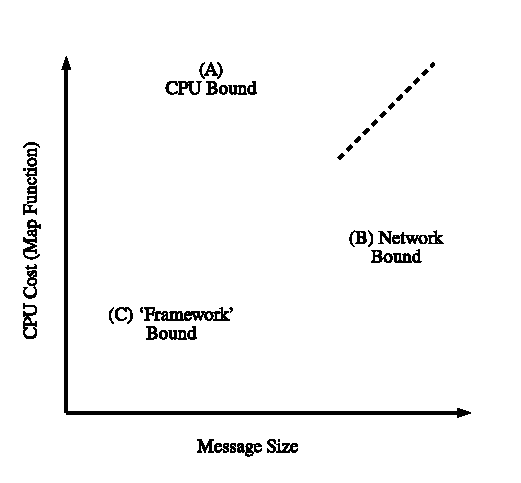
\includegraphics[width=0.5\linewidth]{images/prediction}
\end{center}
\caption{Schematic of parameter space for this study, showing the processing cost of the map function, and the message size.}
%Expected Performance Limiting Factors: (A) Expensive Map Function -- CPU bound, (B) Large messages -- network bound (C) frequency in this region should be high (unless constrained by the framework and integration).}
%-- draw (if non-blocking IO), (c) HarmonicIO? Spark Files? (d) Spark -- TCP? (e) -- microscopy use case, characterized by message size range, and minimum bound on CPU load}
\label{fig:prediction}
\end{figure}
%according to the various bounds. 

%The key research question of this paper is how well the framework configurations under study conform to this model, and in which domains.

%, and where different performance would be expected from the various framework configurations:

\textbf{A - Small message size, large processing cost - CPU Bound}: For sufficiently large processing cost in relation to message size, performance will be CPU bound. Relative performance of the frameworks in this region will be determined by their ability to utilize CPU, and minimizing processing overheads. This regime would be typical of scientific computing applications involving e.g. a simulation step as part of the map stage.
%, and for computationally expensive feature extraction on smaller images.}}% to leave cores free to process messages.
% BB: we're talkimg 1000 bytes here. tweets not images.

%Relative performance will be determined by additional processing needs of each framework.
\textbf{B - Large message size, small processing cost - Network Bound}: For sufficiently large message size, performance will be network bound. In this region, relative performance between frameworks will be determined by the network topology. P2P network topologies should perform well, whereas routing messages among the worker nodes will create additional network traffic which could impair performance. This regime would be typical for scientific computing applications involving relatively simple filtering operations on binary large objects (BLOBs), such as filtering of massive genomics datasets~\cite{ausmeesBAMSIMulticloudService2018}.

% \textbf{B - Large message size, large processing cost}: Here, the performance will be constrained by the minimum of the network and CPU bound, and associated performance on the particular configuration.

\textbf{C - Small messages, small processing cost}: In this regime processing frequency should be high. This region will expose any limitations on the absolute maximum message frequency for the particular integration and thus may be `framework bound'. Well-performing frameworks may be able to approach the network bounds; with very high frequencies. This regime would be typical for the type of enterprise applications studied in previous benchmarks.% such as analysis of social media streams.

\textbf{A-B Boundary Region - Large messages, large processing costs}: Near this boundary (indicated by the dotted line), processing frequency will be low. The large message size means that network speed will bound the overall frequency, whilst high processing costs means that CPU load will also bound the message frequency. Theoretically, the exists a boundary where these two bounds are equal. Overheads in network communication and CPU load will influence exactly where this lies. 

%the framework configurations themselves will the 
%\end{itemize}



%To refine the research question, our methodology will investigate: under what conditions the performance of the framework configuration can approach the theoretical bounds? how closely? and how the relative performance of the farmworker configurations compare across this domain?Indeed, if high performance is limited to a particular sub-domain, what are the bounds? 
%This study attempts to quantify the boundaries where one configuration begins to outperform another.


%Whilst we can make qualitative predictions about which configurations may perform best at in each condition, its hard to estimate how these different factors will influence overall performance across the parameter space. In this study, we quantify (albeit for a particular infrastructure) the boundaries at which one configuration outperforms another, or reaches some particular bound on performance.

% For Apache Spark Streaming (ASS) we’d expect performance for small messages to be highly performant, and hence the bottleneck to be network bandwidth (but we’d expect more CPU usage for smaller messages - as processing cost on the ASS master node will be per-message). Conversely, large messages may highlight potential issues with the engineering of ASS - internal bottlenecks perhaps? - because maybe ASS was never designed for messages $>$1MB.



% (A) If processing cost / message becomes quite high, and messages themselves are reasonably large (say more than 10KB), in this region the pipeline is effectively CPU-bound on the processing nodes, and both frameworks should exhibit similar performance (so long as the threads/node is equal between both platforms)

% (B) if message size (and processing cost) is small, because of the synchronous processing on nodes, and web requests between processes for each message - the latency (albeit small) of these requests will start to have a detrimental impact on the performance of HarmonicIO.
% In the extreme case, the master node will become overloaded with such metadata requests, and will prevent further scaling.

% (C) in such cases, I would expect Spark to perform well, I would expect highly optimized asynchronous IO, and messages are processed in batches. This kind of processing is the intended use case for Spark.

% if message size is sufficiently large, and compute cost is low (this is more like our microscopy case study), we are almost network-bound. In our setup with a single streaming source, performance should be identical between both frameworks, as both are able to reach the maximum throughput of the underlying network (with the message frequency being low).
%(4) if message size is large, and compute cost is low (this is more like our microscopy case study), we are almost network-bound, and HarmonicIOs
%P2P direct streaming architecture should mean it outperforms Spark, as the cost of forwarding such large messages begins to have a negative performance impact.



%%\textcolor{green}{ST: I think it will be better if we bring the figure together with the high-level details a bit early in the article. I mean the figure and the description set the goal for our reader what we are aiming at and what they can expect from this article.} BB: done

\section{METHODOLOGY}\label{method}
%\textcolor{blue}{approach, key decisions. Section for each candidate configuration?}

%As discussed above,
%Our goal is to
%{\color{red}{AH Repetitive. Remove?? We investigate the performance of HarmonicIO and Apache Spark (under various configurations), under a full range of application loads, including those typical of more scientific use cases such as our specific application - microscopy image processing. Building on previous studies that have tended to focus on small messages, with low processing cost associated with each message, }}

Varying message size (100 bytes -- 10MB), and CPU cost for processing each message (0 -- 1 second per message)
%With our tunable experimental setup, for each iteration of the experiment, 
%We vary (a) the size of the messages, and (b) the CPU cost per message to sweep the parameter space -- and for each parameter pair, 
allowed us to sample the performance of the studied streaming frameworks over a parameter space with settings ranging from highly CPU-intensive workloads to highly data-movement intensive use-cases. This domain captures typical enterprise use cases, and scientific computing workloads.

%, and sample performance of the streaming frameworks to evaluate their performance. 


%we use our tools to find the maximum  for each of the three parameter spaces, 
%This parameter sweep approach means that we can evaluate the expected performance of the system for a wide range of applications and use cases (in contrast to other studies).

%To build on previsou studies by building a more complete picture of the performance characteristics, 

%We vary the message size (), and CPU cost ().
The microscopy use case is a particular focus: message (image) sizes 1-10MB, with a CPU cost profiled at around 100mS for very simple analysis (consistent with \cite{torruangwatthanaHarmonicIOScalableData2018a}) -- CPU cost would depend on the specific features being extracted, and could be significantly higher.
%-- in particular, at scale with large ($>$1MB), or very large (\textasciitilde10-100MB) message sizes?
We measure maximum sustained frequency (i.e throughput, messages per second) at each point (message size, CPU), for HarmonicIO, and each of the Spark stream source integrations explained below:%, so that we get an overview of performance limits of the various frameworks (and integrations) as a function of these input parameters.
%The implementation of the benchmarking tools is explained in the next section.

% We use the developed benchmarking tools to



% decision to measure throughput
% These 
% factors, choice of param space -- microscopy use case
% %\textcolor{blue}{  What will we vary}
% Number of factors which affect the performance (for a given architecture):

% \begin{itemize}
% \item "constant factors": network speed, CPU speed etc, (changes to these are hard to factor in)
% \item "input factors": size of message, processing cost / message (+ comms to other services)
% \item "output factors": throughput (we choose to fix the number of nodes, and measure the maximum throughput)
% \end{itemize}

%For a complete picture of the performance 

%\subsection{Apache Spark Streaming Source Integrations}

%There are many possible stream integrations for Apache Spark Streaming -- we discuss some of the most common, likely to be adopted by new users:
%We exclude more complex integration options such as the \texttt{RawInputDStream} -- requiring more detailed knowledge of Spark. These input integrations were chosen:



%We focused on low-level integrations (offering minimal abstraction on top of the operating system) -- this simplicity should make it easier to analyze performance characteristics. 

%Furthermore, using low-level abstractions make it easier for scientists to integrate existing or legacy applications for use with the framework, without the need for additional software development\footnote{On this basis, we exclude more complex integration options such as the \texttt{RawInputDStream} -- requiring more detailed knowledge of Spark.}. 
%This is a key concern in a scientific computing context, where software needs teb e
%Secondly, we avoided middleware requiring dedicated compute resources, so that we could compare fairly on a hardware-utility basis with more low-level approaches, and to avoid additional  configuration and deployment complexity. Fewer layers means the pipeline is perhaps better able to ``keep the data moving'' -- one of the ``eight rules for real-time stream processing''~\cite{stonebrakerRequirementsRealtimeStream2005a}.



%. With these goals in mind, we selected input sources for ASS:

\textbf{Spark + TCP Socket:} TCP sockets are a simple, universal mechanism, easy to integrate into existing applications, with minimal configuration. 
%Being a low-level abstraction, it gives us more transparency when investigating how well ASS can utilize the network hardware. 

% Simple to model, less clouding of performance characteristics. True P2P (but only 1:1). no additional hardware. 
% A simple, low-level integration: its easy to create a streaming server able to stream over a TCP socket; such a setup is similarly advantageous to integrate into scientific applications more generally (as it requires no dependence on Spark libraries.) This simple setup will make it easier to understand the performance characteristics, and will hopefully allow good use of all available network bandwidth. This configuration requires no additional infrastructure nor hardware. Whilst allowing a `direct' connection between stream source (helping to 'keep the data moving' --- cite 6 rules), so whilst a P2P with many sources (i.e. read parallelism) is possible the application must be specifically configured for each source.

\textbf{Spark + Kakfa:} Kafka is a stream processing framework in its own right: Kafka producers write messages onto one end of message queues, which are processed by Kafka \emph{consumers}. 
%These messages queues are organized by topic, and by partition -- so that a single logical message queue can be distributed between nodes (offering resilience), with messages written to disk for durability. 
Kafka is commonly used in conjunction with Spark Streaming in enterprise contexts, to provide a resilient and durable buffer, allowing Spark applications to be restarted without interrupting the streaming source. We deploy a single Kafka server as this most resembles the HarmonicIO deployment. 
The newer \emph{Direct DStream} integration approach with Kafka is used in this study. Under this integration, messages are transferred directly from the Kafka server to Spark workers.

\textbf{Spark + File Streaming:} Under this approach, Spark will process new files in each batch interval. % offering an ostensibly straightforward approach to integration. 
%Rather than using HDFS (for reasons described below), 
We configure an NFS share on the streaming source node. This allows direct transfer of file contents from the streaming source node, to the processing machines -- similar to the TCP socket approach used in HarmonicIO. 
% we use the file system as the integration boundary (to achieve this in a networked context, we use NFS shares).
% Again, a simple approach, easy for new users to configure, requiring minimal knowledge of Spark internals. NFS is intended to be used for file transfer over or a local network, for the file sizes we're working with. NFS should allow direct transfer of file data between source and processing nodes (with good performance -- mirroring HarmonicIO's architecture in that regard).
%, the performance of the file listing over the network may have a performance impact in some cases.
% \textbf{Spark + File Streaming (with NFS) [TICK]:}
% %: True P2P. simple(r), less clouding of performance characteristics. no additional hardware (fairness), utility.
% For a fair comparison with HarmonicIO, we wanted to focus on direct data transfer, with simple configurations to make it possible to understand the performance characteristics. We wanted to explore use cases that are network-bound in terms of data ingress. To that end, we decided to investigate the performance of NFS shares on the streaming source node (mounted on the Spark cluster), as a way of achieving more direct file transfer, whilst integrating with Spark. 
% Note that this approach still uses the HDFS \emph{drivers}, to work with the local file system in so-called \emph{raw} mode\footnote{without using full HDFS.}.
% This approach more closely resembles HarmonicIO's P2P architecture, in way that allows adding and removing of streaming sources in a way that is transparent to the streaming application -- the file system can function as a layer of abstraction -- Spark can watch a folder (by repeated directory listing), within which we can mount NFS shares for different streaming sources, while the application is running. Multiple streaming sources is a use case we intend to investigate in future work. 
We do not use HDFS, a distributed filesystem intended replicated storage of very large (append-only) files -- many GBs; TBs, this makes it inappropriate for the files used in this study, which are at most 10MB. 
Indeed, other distributed filesystems wouldn't offer us the P2P message transfer. Nor did we not use Cassandra, a distributed wide-column store, as we exceed the "single digits of MB" being suggested as a sensible limit~\cite{CassandraLimitationsCASSANDRA2Apache}. 

%Conversely, some typical integration approaches we decided not to include in this study:
%\textbf{File Streaming (with HDFS):} HDFS is a distributed file system, its core functionality is to manage partitioning and replication of very large files across storage nodes, for read performance and durability -- constituting a distributed file system.
%However, HDFS is append-only, and intended for very large files . It is not intended for handling small files, and reading and writing files to disk (with replication) requires additional hardware, creates complexity, and would confound our interpretation of Sparks performance characteristics.

%\textbf{Spark + Kafka:} Kafka~\cite{kreps2011kafka} is a distributed transaction log (or distributed ledger)
%\footnote{Kafka has began offering some basic stream processing functionality of its own -- \emph{Kafka Streams}.}, 
%and is frequently used in conjunction with frameworks such as Spark, to act as a queue or buffer for incoming messages -- an advantage of such an architecture is that revised versions of Spark applications can be redeployed without data loss. 
%Kafka is a complex framework in its own right, requiring deployment and configuration of services such as ZooKeeper~\cite{Junqueira:2013:ZDP:2904421}. Importantly, Kafka is intended for small message sizes\footnote{In its default configuration, it will reject any messages larger than 1MB.} -- it is a distributed message log, not a distributed file system, and will undoubtedly have its own performance characteristics which would confuse our analysis of Spark.

%\subsection{HarmonicIO}
%\textcolor{blue}{ Why HarmonicIO?}




% , providing an interesting comparison with other streaming processing architectures

\section{EXPERIMENTAL SETUP \& BENCHMARKING TOOLS}\label{expsetup}

\begin{figure*}[h]
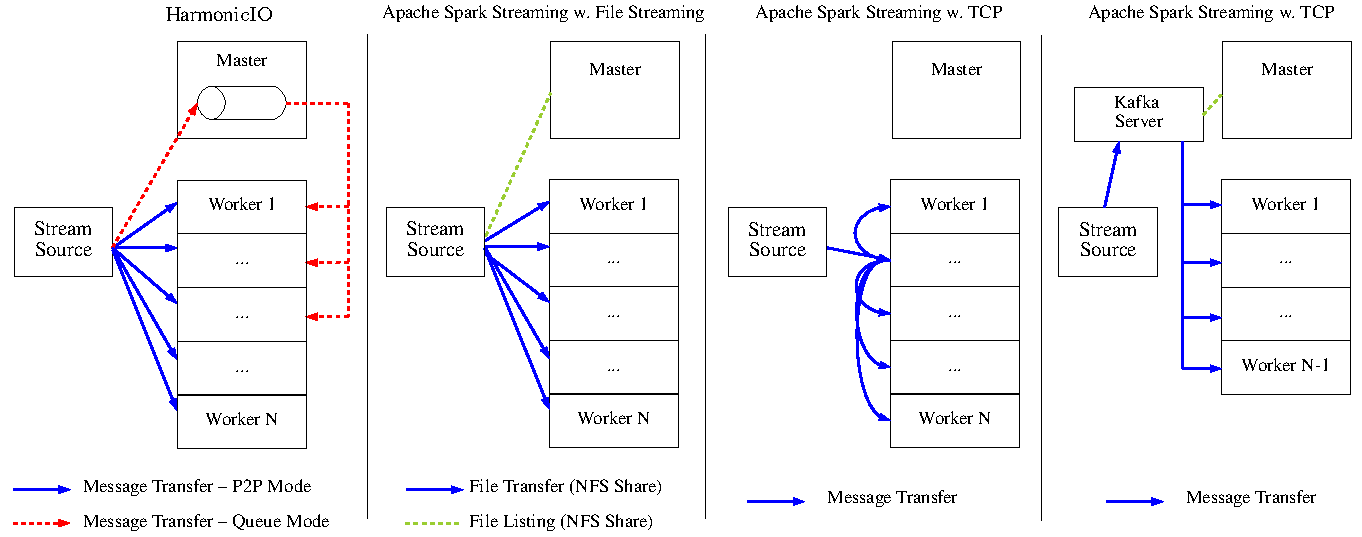
\includegraphics[width=\textwidth]{images/arch-comp-w-kafka}
\caption{Architecture / Network Topology Comparison between the frameworks and streaming source intregrations -- focusing on major network traffic flows. Note that with Spark and a TCP streaming source, one of the worker nodes is selected as `receiver' and manages the TCP connection to the streaming source. 
Note that neither the monitoring and throttling tool (which communicates with all components) are shown, nor is additional metadata traffic between nodes (for scheduling, etc.). Note the adaptive queue- and P2P-based message processing in HarmonicIO.}
\label{fig:arch-comp}
\end{figure*}


To explore the (message size, CPU cost per message) parameter space we developed benchmarking tools\footnote{Available at: \url{https://github.com/HASTE-project/benchmarking-tools}} for Spark and HarmonicIO, able to process synthetic messages, and generate synthetic CPU load.
%{\color{red}{AH: Does not agree with actual figure.} }
Fig.~\ref{fig:arch-comp} shows the various pipelines showing of HarmonicIO, and Apache Spark Streaming with file, Kakfa and TCP based integrations. The arrows show the busy network communication.
%(a) streaming server (b) a cluster of processing nodes and (c) a monitoring and throttling tool to orchestrate the experimental work, and aggregate performance metrics.
%For a fair comparison, 
For each setup, 6 stream Processing VMs were used, each with 8 VCPUs and 16GB RAM (1 master, 5 workers). For the streaming source VM we used a 1 VCPU, 2GB RAM instance.  
%When measured with iperf, network performance was 1.4 Gbps.
These resources are similar to the experimental setup of \cite{xinApacheSparkFastest2014}, where 40 cores were used.
%We used a tenant-based private network to be consistent with throughput. 
The maximum network bandwidth monitored using \texttt{iperf} was 1.4Gbit/s. 
Ansible scripts used to deploy the cluster are at: \url{https://github.com/HASTE-project/ansible-benchmarking}.

% ST code?
% BB: ST: this repeats these
%For HarmonicIO we have setup a virtual cluster of six nodes, one master and five workers nodes. 
%Each node in the cluster was a $ssc.xlarge$ virtual machine consisted of 8 VCPUs, 16GB RAM and 160GB local disk. 
Below, we describe the details of the experimental setup for each framework, and the approach used for determining the maximum frequency message throughput.

\subsection{Apache Spark}
%For subsequent parameter exploration, we needed tunable message size and CPU load -- necessitating a separate simulator, and stub application. 


We created a \emph{streaming source} application, supporting TCP and file-based streaming modes in ASS. 
Each message is the CPU pause (as a string), padded up to the specified message length, so that both parameters (CPU load and message size) can be tuned via the streaming source application. 

Inside the application, we used the \texttt{getThreadCpuTime()} method of the \texttt{ThreadMXBean}\footnote{\url{https://docs.oracle.com/javase/7/docs/api/java/lang/management/ThreadMXBean.html}} from JavaSE, which returns the total time spent executing by the thread in both user and system mode (excluding blocked and waiting times), polling this until the `CPU load' parameter from the message has elapsed. Hence, we simulate a CPU-intensive message processing step. Consequently, our benchmark has the effect of revealing the CPU overhead of the different frameworks and integrations. 


%Neither mode has built-in auto-throttling (backpressure? look up docs) functionality, 
% its unclear (to me) whether file and TCP streaming support backpressure, and if they do, how it would work in practice. Better just not to mention backpressure -- our goal is to find the max throughput.
% Maybe bad decision? :(
% https://www.slideshare.net/SparkSummit/reactive-streams-linking-reactive-application-to-spark-streaming
To determine the maximum throughput, we adopt the approach of gradually increasing the message frequency (for a fixed (message\_size, CPU cost) pair) until a bottleneck is detected somewhere in the pipeline, then a binary search to find the maximum. A monitoring and throttling tool was developed for this purpose. Listing~1 shows a simplified view of the algorithm used to determine the maximum. To achieve this, it monitors and controls our streaming source application and the spark application, through a combination of REST APIs and log file analysis. 
%This requires several hundred hours of clock time, so inevitably the tool needed to be restarted: the tool is able to resume `where it left off'. 
%The benchmarking tool saves progress so that it can be restarted over several days. 
%The tool is also able to restart the Spark application, Spark itself, Kafka when they fail during 



% Maximum throughput frequency (for given message size, cpu load) is determined as follows:
% so a further 'throttling' application, will, for a given (message\_size,CPU cost) pair tune the streaming server remotely to gradually increase the message frequency, until a bottleneck is is detected. 

% TODO: not a figure

%%\textcolor{green}{ST: Perhaps we can use a pseudocode version of this code, will take less space.} BB: squashed it.




% \begin{lstlisting}[
%   caption={Monitoring and Throttling Algorithm (Simplified). Until an upper bound is reached, increase piecewise linearly, then binary search.}
%   label=listing:throttle,
% ]

\begin{figure}
\centering
\begin{scriptsize}
\begin{verbatim}
def find_max_f(msize, cpu_cost):
    max_known_ok_f <- 0
    min_known_not_ok_f <- null
    f <- f_last_run or default(msize, cpu_cost)
    while true:
        metrics = [spark_metrics(), strm_src_metrics()]
        switch heuristics(metrics):
        case sustained_load_ok: 
            f <- throttle_up(metrics, f)
        case too_much_load:
            f <- throttle_down(f)
        case wait_and_see:
            pass
     sleep

def throttle_up(metrics, f):
    max_known_ok_f <- f
    if min_known_not_ok_f == null:
        load = estimate_fraction_max_load(metrics)
        if load < 0.01: new_f <- f * 10
        elif load < 0.1: new_f <- f * 5
        elif load < 0.5: new_f <- int(f * 1.10)
        elif load < 0.8: new_f <- int(f * 1.05)
        else: new_f <- int(f * 1.05)
        if f == new_f:
            new_f <- f + 1
        return new_f
    else:
        return find_midpoint_or_done()

def throttle_down(f):
    min_known_not_ok_f <- f
    return find_midpoint_or_done()

def find_midpoint_or_done():
    if max_known_ok_f + 1 >= min_known_not_ok_f: 
        done(max_known_ok_f);
    else: 
        return int(mean(max_known_ok_f, 
                        min_known_not_ok_f))

\end{verbatim}
\end{scriptsize}
\caption*{Listing 1: Monitoring and Throttling Algorithm (Simplified). Until an interger upper bound is reached, increase piecewise linearly, then binary search.}
\end{figure}
%\end{lstlisting}

% This trial and error approach differs from the backpressure mechanism, in that it is able to (a) consider a broader set of metrics than the total delay, and (b) assumes linearity only to estimate the max throughput, and will continue to throttle up until the application fails, to accurately find the true maximum throughput.
% https://www.slideshare.net/SparkSummit/reactive-streams-linking-reactive-application-to-spark-streaming

% Progress is recorded, so we restart where we left off in case of failure.


This process is repeated for (message\_size, CPU cost) in a parameter sweep. 
We used a batch interval of 5 seconds, and a micro-batch interval of 150mS. Experimenting with other values had little impact on throughput. For the Spark File Streaming investigation, files are shared on the streaming server with NFS. %, and the share is mounted on all the processing machines.
%For TCP streaming, we use the default replication level. (TCP are 'recoverable', so replication is enabled by default to give data resiliance incase of node failure).
Maximum throughput is reached when a bottleneck occurs somewhere in the system, as detected by the throttling tool:
\begin{itemize}
\item ASS taking too long to process messages.% (i.e. `Total Delay' exceeds the batch interval -- the key spark performance metric for stream processing). This can be due to a combination of network and/or CPU bound performance.
\item There is a network bottleneck at the stream source.%, the source application reporting it cannot stream messages sufficiently.% (in the TCP 
\item For file streaming, ASS is taking too long to perform a directory listing.% to decide which files to include in the next batch (this depends on the performance of NFS, the HDFS drivers, caches, and the way the file system is queried) 
%FILE\_LISTING - Spark is taking too long to list the files to be included in the next batch. (this shares the same network connection). Used caching in NFS client, etc. etc.
%LIMIT\_STREAM\_SRC -- 
%streaming case).
\end{itemize}

%The bottleneck can be one of:

%Determining the precise nature of the underlying bottleneck is non-trivial, when visualized, we see results conforming to theoretical CPU and network bounds.

% For simplicity, we use the original Apache Spark Streaming API (not the newer Structured Streaming API).


\subsection{HarmonicIO}
%For HarmonicIO we did %\textcolor{blue}{ST -- what did you do?...}

%For HarmonicIO, the maximum throughput is easier to determine, since the HarmonicIO streaming client is synchronous for message transfer (multiple client threads are used to obviate negative performance impact).
%-- meaning that it will self-regulate. 
In HarmonicIO, the maximum throughput is determined by measuring the time to stream and process a predefined number of messages for the given parameters. 
We created a separate benchmarking application for HarmonicIO, which reads messages in our format. As with Spark, metadata describing the amount of CPU load is embedded in each message. 
The message size in the HarmonicIO benchmark application varies up to 10MB, representing the large individual messages within the scientific datasets. The range of the message sizes covers scientific datasets based on multidimensional arrays, binary blobs and text-based datasets. For CPU load, we have used an artificial workload of different durations. See section IX.


%Each worker hosted 8 Processing Engine containers that in total contributed 40 processing slots (one for each core). %based on a cluster of $5$ workers. -- we said this above

%A single client virtual machine with multi-threading application (using Python module $multiprocessing$) was used for data streaming. 
%The client application used six independent threads with equally distributed workload.     
%For HarmonicIO, we read from memory (pre-caching from disk) and store in MongoDB. \te
%- HarmonicIO: multi-threaded (TODO: push to github?)

\section{RESULTS}\label{results}

% \begin{figure}[h]
% %[width=0.9\textwidth]
% \begin{center}
% %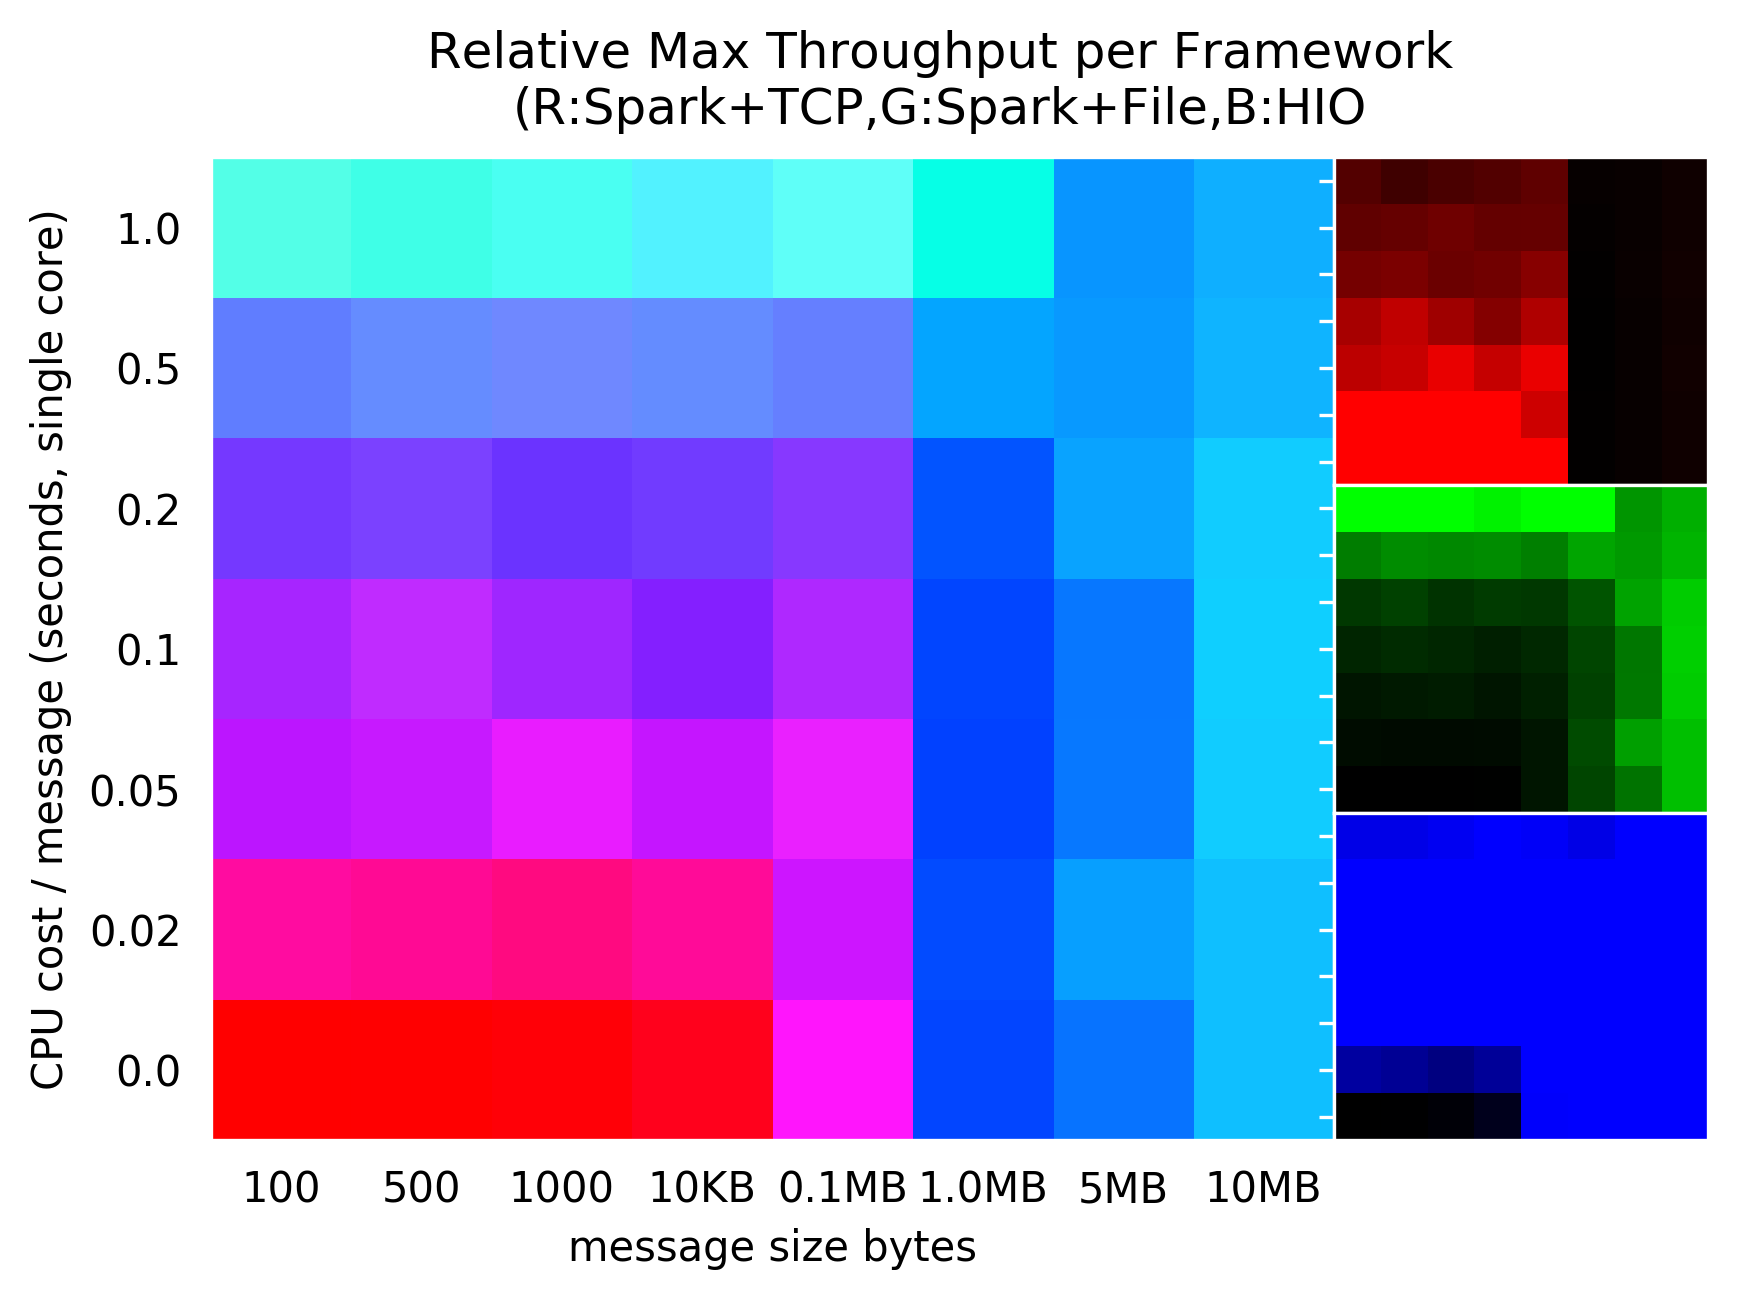
\includegraphics[width=9cm]{images/3_cases_rgb.png}
% 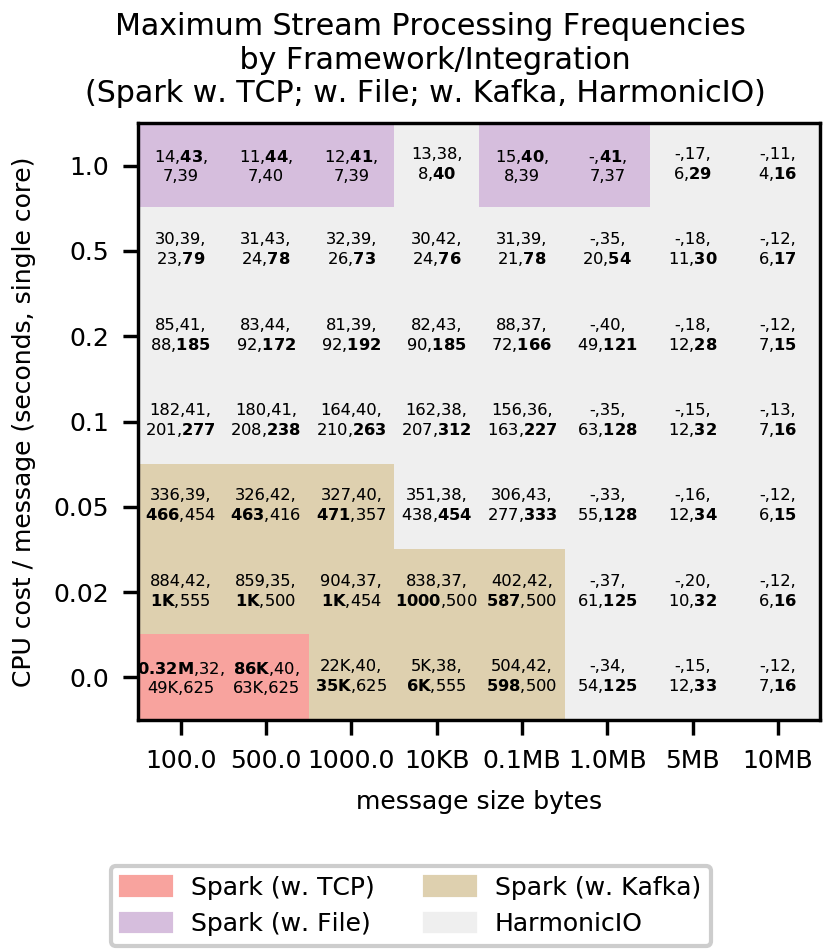
\includegraphics[width=8cm]{images/best-w-freqs-cropped.png}
% \end{center}
% \caption{Performance of Apache Spark (under TCP, File streaming, and Kafka integrations), and HarmonicIO, by maximum message throughput frequency over the domain under study. Under each setting, the highest frequency is shown in bold, with color-coding according to which framework/integration was able to achieve the best frequency. Compare with Fig.~\ref{fig:prediction}.}
% \label{fig:blobs}
% \end{figure}


%%%%%% modifications by Salman %%%%%
\begin{table*}
\setlength{\tabcolsep}{2pt}
% \small
\fontsize{8pt}{8pt}\selectfont
\begin{center}
\renewcommand{\arraystretch}{1.4} % Default value: 1
\begin{tabular}{|l||c|c|c|c|c|c|c|c|}
\hline 
\multicolumn{9}{ |c| }{Maximum Message Frequency (Hz) [Apache Spark with TCP, Apache Spark with File streaming, Apache Spark with Kafka, and HarmonicIO]} \\
\hline 
CPU Cost & \multicolumn{8}{ |c| }{Message Size (bytes)} \\
\hline
 & 100  & 500  &  1000 &  10KB &  0.1MB  & 1.0MB & 5MB & 10MB \\ \hline \hline

1.0 secs  & 14, \textbf{43}, 7, 39 & 11, \textbf{44}, 7, 40 & 12, \textbf{41}, 7, 39 & 13, 38, 8, \textbf{40} & 15, \textbf{40}, 8, 39 & -, \textbf{41}, 7, 37 & -, 17, 6, \textbf{29} & -, 11, 4, \textbf{16} \\
\hline

0.5 secs  & 30, 39, 23, \textbf{79} & 31, 43, 24, \textbf{78} & 32, 39, 26, \textbf{73} & 30, 42, 24, \textbf{76} & 31, 39, 21, \textbf{78} & -, 35, 20, \textbf{54} & -, 18, 11, \textbf{30} & -, 12, 6, \textbf{17} \\
\hline

0.2 secs  & 85, 41, 88, \textbf{185} & 83, 44, 92, \textbf{172} & 81, 39, 92, \textbf{192} & 82, 43, 90, \textbf{185} & 88, 37, 72, \textbf{166} & -, 40, 49, \textbf{121} & -, 18, 12, \textbf{28} & -, 12, 7, \textbf{15} \\
\hline

0.1 secs  & 182, 41, 201, \textbf{277} & 180, 41, 208, \textbf{238} & 164, 40, 210, \textbf{263} & 162, 38, 207, \textbf{312} & 156, 36, 163, \textbf{227} & -, 35, 63, \textbf{128} & -, 15, 12, \textbf{32} & -, 13, 7, \textbf{16} \\
\hline

0.05 secs  & 336, 39, \textbf{466}, 454 & 326, 42, \textbf{463}, 416 & 327, 40, \textbf{471}, 357 & 351, 38, 438, \textbf{454} & 306, 43, 277, \textbf{333} & -, 33, 55, \textbf{128} & -, 16, 12, \textbf{34} & -, 12, 6, \textbf{15} \\
\hline

0.02 secs  & 884, 42, \textbf{1K}, 555 & 859, 35, \textbf{1K}, 500 & 904, 37, \textbf{1K}, 454 & 838, 37, 1K, 500 & 402, 42, \textbf{587}, 500 & -, 37, 61, \textbf{125} & -, 20, 10, \textbf{32} & -, 12, 6, \textbf{16} \\
\hline

0.0$\dagger$ secs  & \textbf{0.32M}, 32, 49K, 625 & \textbf{86K}, 40, 63K, 625 & 22K, 40, \textbf{35K}, 625 & 5K, 38, \textbf{6K}, 555 & 504, 42, \textbf{598}, 500 & -, 34, 54, \textbf{125} & -, 15, 12, \textbf{33} & -, 12, 7, \textbf{16} \\
\hline

\end{tabular}
\end{center}
\caption{Maximum Message Processing Frequencies of Apache Spark (under TCP, File streaming, and Kafka integrations), and HarmonicIO; in that order. These results are visualized in Fig.~\ref{fig:blackblobs}. There is no data for Spark + TCP for message sizes of 1MB or more, as it did not perform reliably in this domain. The highest message frequency in each case is shown in bold. $\dagger$ 0.0 denotes nil CPU load.}
\label{table:results}
\end{table*}
%%%%%%%%%%%%%%%%%%%%%%%%%%%%%%%%%%%%

\begin{figure}[h]
%[width=0.9\textwidth]
\begin{center}
%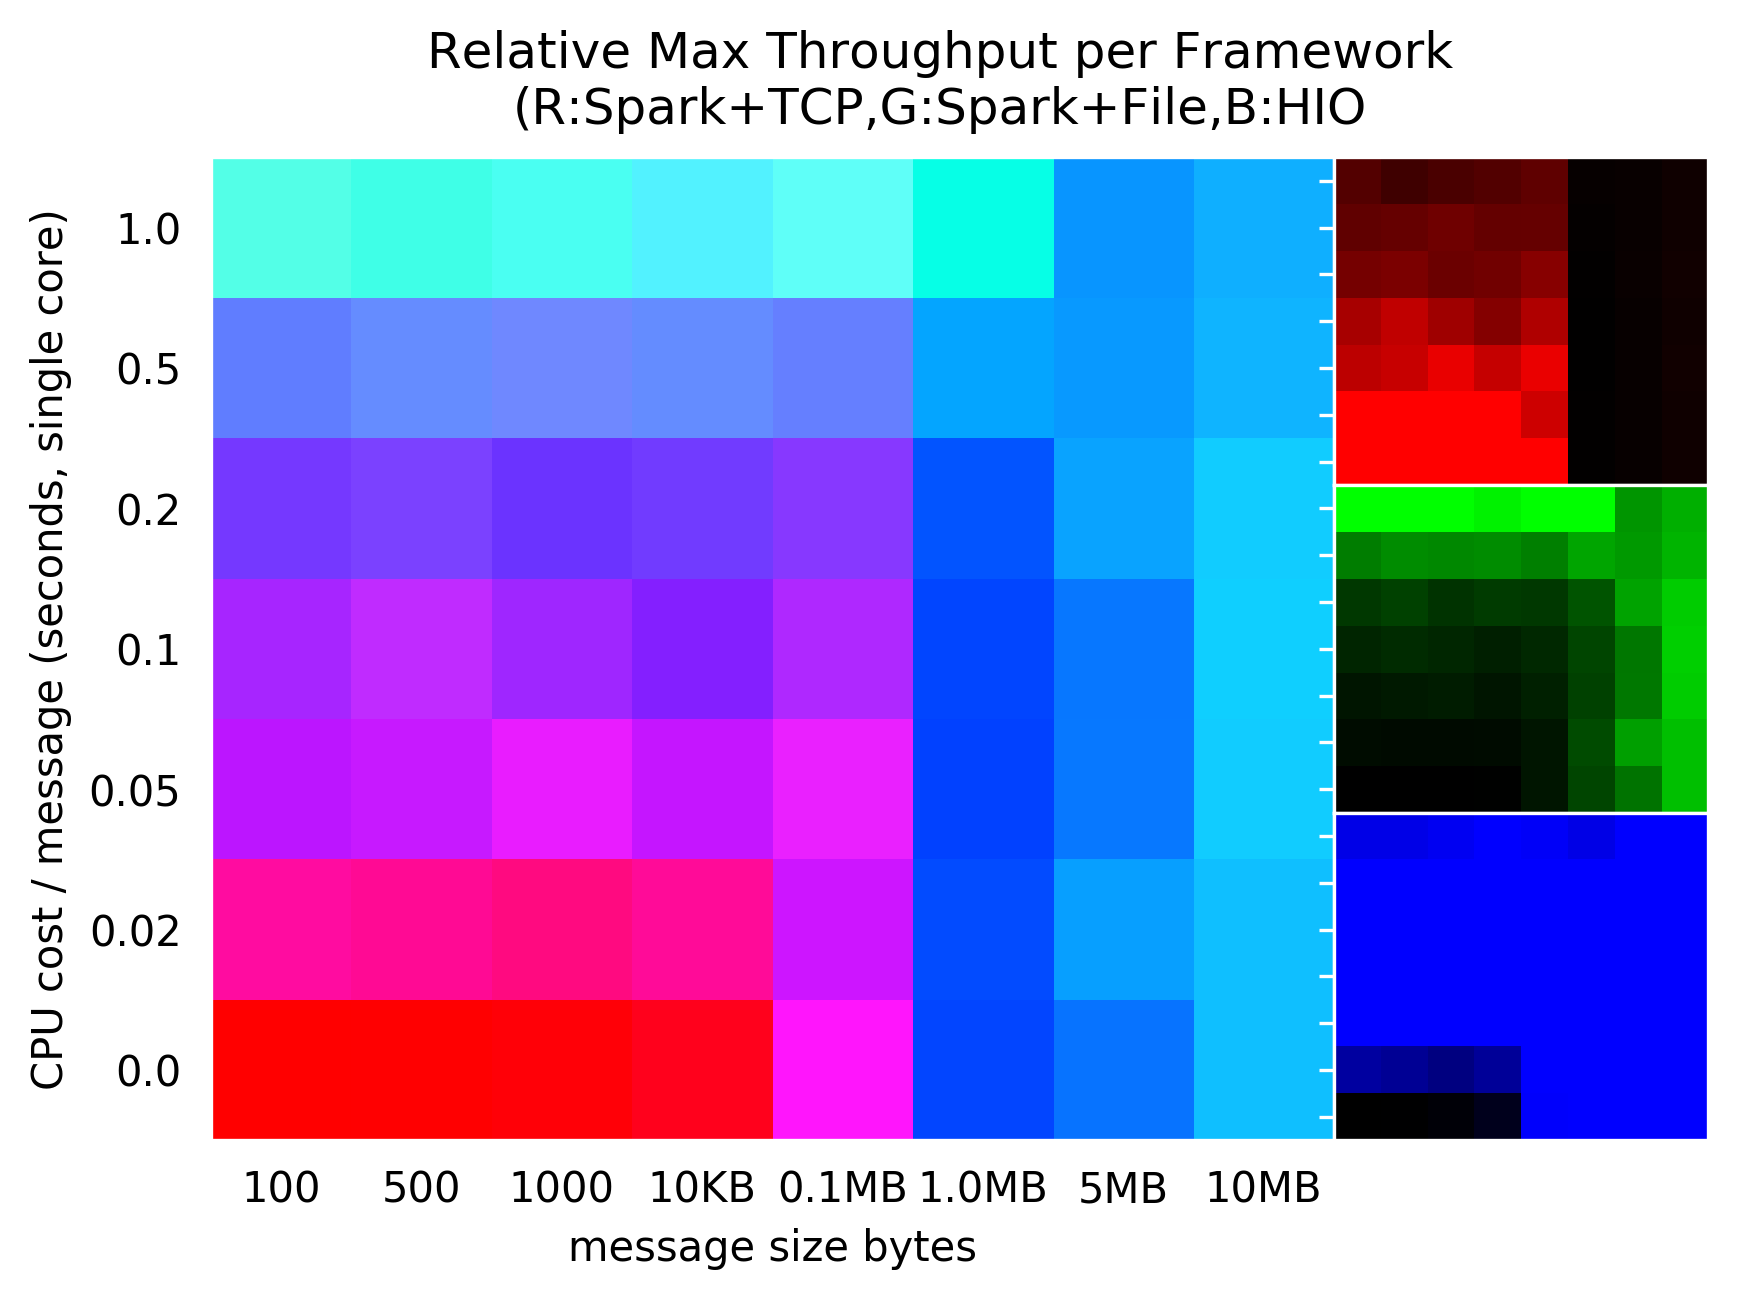
\includegraphics[width=9cm]{images/3_cases_rgb.png}
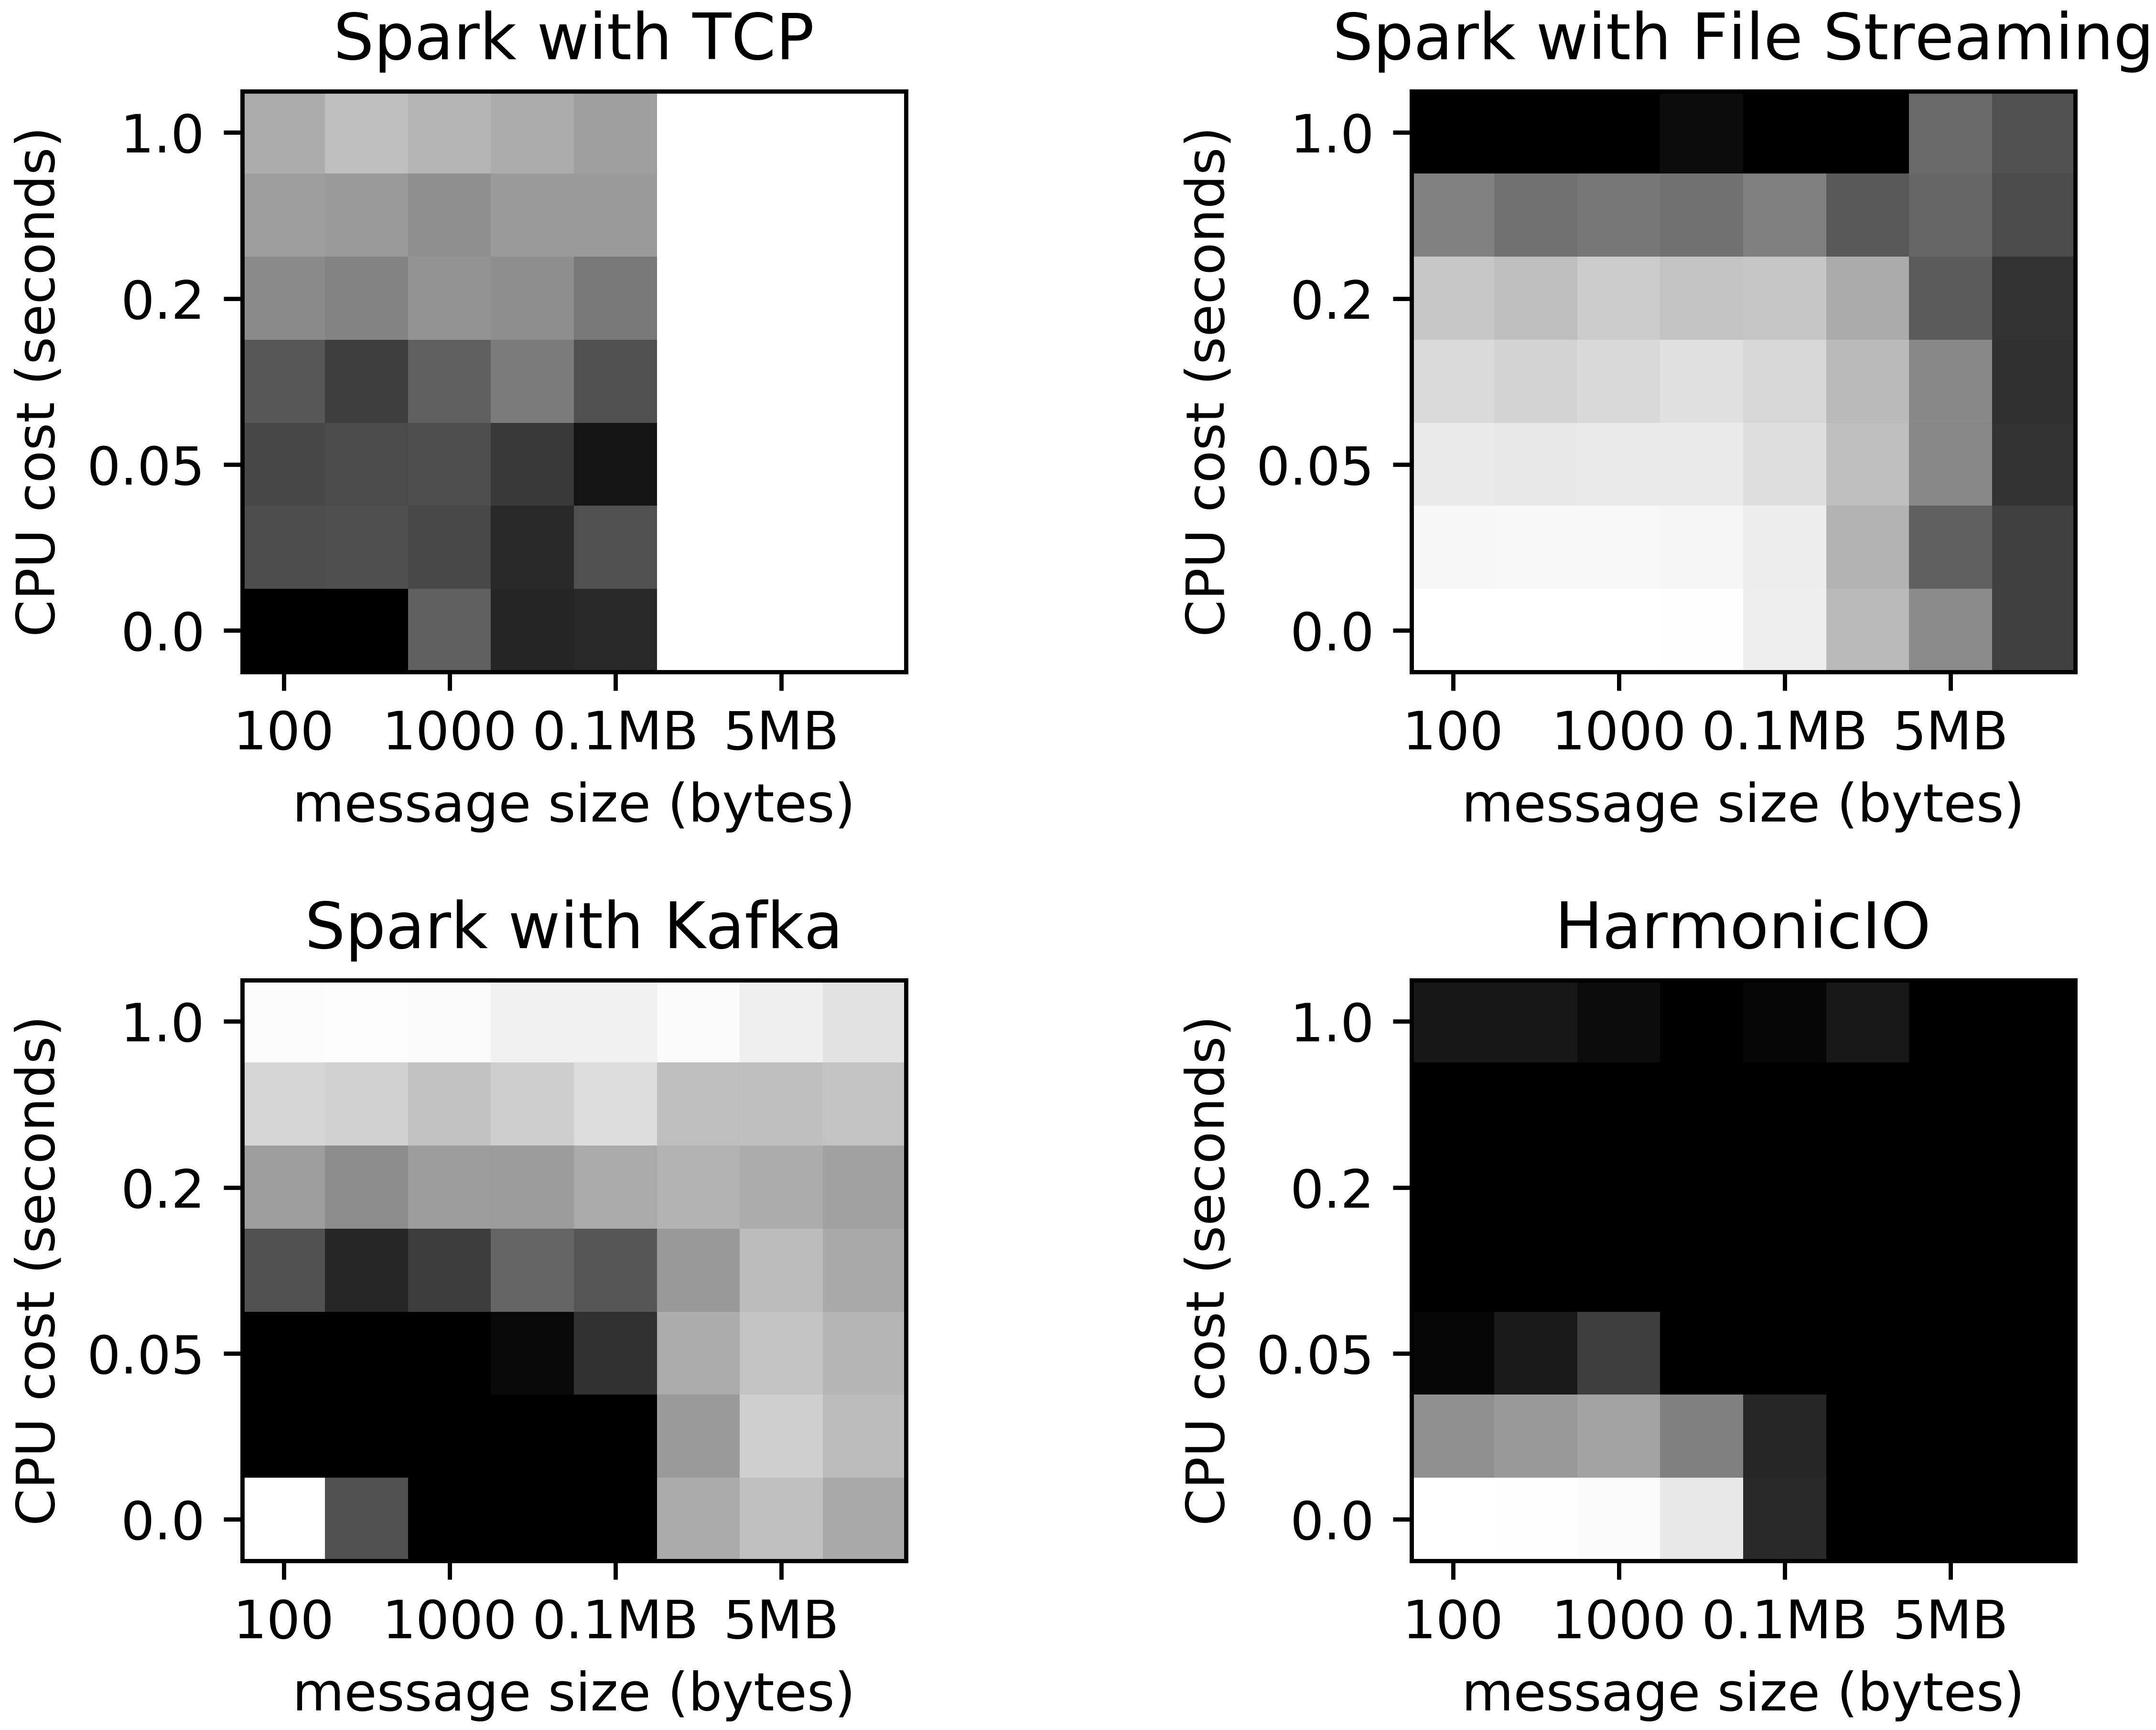
\includegraphics[width=8.25cm]{images/4-greyscales.png}
\end{center}
\caption{Performance of the frameworks and stream integrations over the domain under study. 
The brightness represents the message frequency as a fraction of the best performing framework at that position --
completely dark areas indicate where the respective framework was the best performing, lighter areas indicate lower message frequency. Compare with Fig.~\ref{fig:prediction}. There is no data for Spark + TCP for message sizes of 1MB or more, as it did not perform reliably in this domain.}
\label{fig:blackblobs}
\end{figure}



% figure* for 2-col, see: https://tex.stackexchange.com/questions/30985/displaying-a-wide-figure-in-a-two-column-document
\begin{figure*}[h]

\begin{center}
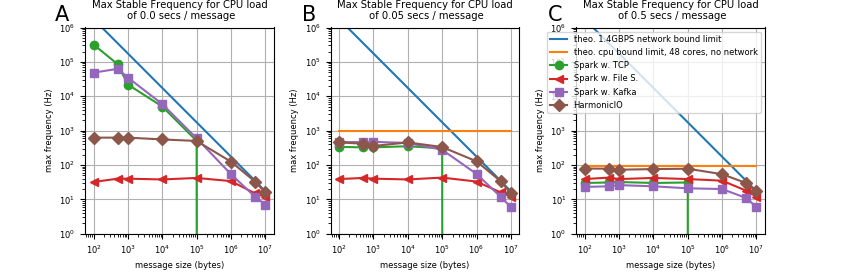
\includegraphics[width=0.9\textwidth]{images/selected_simple_plots.png}
\end{center}
\caption{Maximum stream processing frequencies for Spark (with TCP, File Streaming, Kafka) and HarmonicIO by message size; for selection of CPU cost/message.}
\label{fig:all-results}
\end{figure*}

\begin{figure}[h]
%[width=0.9\textwidth]
\begin{center}
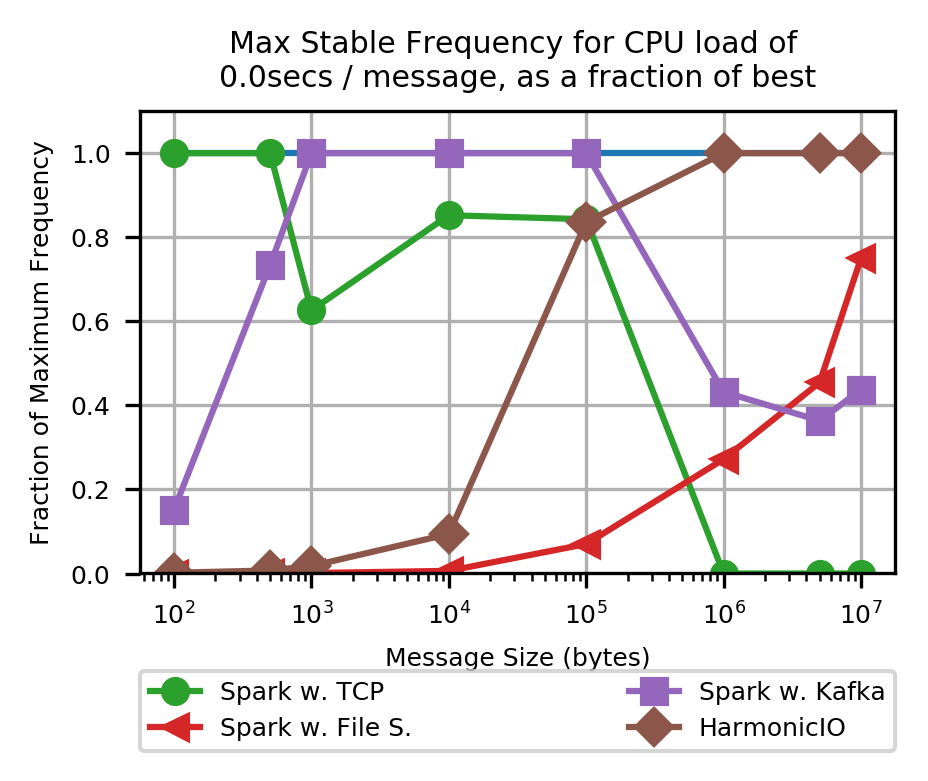
\includegraphics[width=7cm]{images/normalized_0.png}
\end{center}
\caption{Maximum frequency by message size, for Spark (with TCP, File Streaming, Kafka) and HarmonicIO under varying message size; normalized as a fraction of the best performing framework for the particular parameter values.}
\label{fig:result-normed}
\end{figure}


% Per-Framework... SUMMARIES....
%In this section, we compare the relative performance of the frameworks with one another, and with theoretical bounds on network and CPU usage (and how well each framework is able to utilize resources in those cases), and discover trends and other characteristics across the breadth of the parameter space -- these results are discussed later, in Section~\ref{discussion}.
The maximum frequencies achieved by each framework (and stream integration setup), according to message size and per-message CPU load, are show in Fig.~\ref{fig:blackblobs} and Table~\ref{table:results}, color-coded according to the best performing framework. 
A subset of these results is presented again in Fig.~\ref{fig:all-results} and Fig.~\ref{fig:result-normed}, where results for particular CPU loads are shown in relation to CPU and network-theoretical bounds.
%In , some of these results are shown normalized as a fraction of the theoretical bound. 

We summarize the results for each setup, before further discussion in relation to the intended use cases, architectures, and relation to theoretical bounds:% in the proceeding discussion section (\ref{discussion}).

\textbf{Apache Spark Streaming with TCP}: 
This integration achieves very high frequency when message size and CPU load are small, consistent with previous studies. For 100 byte messages without CPU load; the pipeline was able to process messages at frequencies approaching 320KHz, meaning around 1.6M messages were processed by Spark in a 5 second batch. This can seen in the extreme lower-left of Fig.~\ref{fig:blackblobs}, and the results shown in Fig.~\ref{fig:all-results}.A. 
But performance degraded rapidly for larger message sizes, and under our benchmarks, it couldn't reliably handle messages larger than $10^5$ bytes at any frequency.

\textbf{Apache Spark Streaming with Kafka}:
This streaming pipeline performed well for messages less than 1MB, and CPU loads  less than 0.1 second/message, at the bottom-left of Fig.~\ref{fig:blackblobs}. Away from this region, performance degrades relative to other setups in this study, falling away from theoretical limits.

\textbf{Apache Spark Streaming with File Streaming}: 
This integration performed efficiently at low frequencies -- in regions tightly constrained by network and CPU-theoretic bounds (the top and right of Figs.~\ref{fig:prediction} and \ref{fig:blackblobs} and, and the results for higher message sizes in Fig.~\ref{fig:all-results}).

\textbf{HarmonicIO}:
Fig.~\ref{fig:blackblobs} shows that HIO was the best performing framework for the broad intermediate region of our study domain, 
for medium-sized messages (larger than 1.0MB), and/or CPU loads higher than 0.05 seconds/message. It matched the performance of file-based streaming with Apache Spark for larger messages and higher CPU loads.% (the top and right edges of Fig.~\ref{fig:blackblobs}), and the results for larger message sizes shown in Fig.~\ref{fig:all-results}. 

\section{DISCUSSION}\label{discussion}

\subsection{Performance: Message Size \& CPU Load}

% Per-Region... SUMMARIES....Good performance...

%Having discussed the results in summary
%Building on the results summary in the preceding section, this section compares performance among framework configurations, and with theoretical bounds, in the different regions of our study domain. These regions represent different use cases, and each framework setup shows good performance for their own intended use case/region. 

%There are both network- and CPU-bounds on the overall message throughput. 
%Theoretically, 
Maximum message throughput is bound by network and CPU bounds, which are inversely proportional to message size and CPU cost respectively (assuming constant network speed, and number of CPU cores; respectively). The relative performance of different frameworks (and stream integrations) depend on these same parameters. Fig.~\ref{fig:blackblobs} shows that all frameworks also have specific, well-defined regions where they each perform the best. We discuss these regions in turn, moving outwards from the origin of Fig.~\ref{fig:blackblobs}.
%Looking at the figures, the performance landscape over vary message size and CPU load is complex, with each framework/integration performing well under some conditions and poorly on others:

% 1 / 2
Close to the origin, theoretical maximum message throughput is high, Fig.~\ref{fig:all-results}.A shows that for the smallest of messages, Spark with TCP streaming is able to outperform Kafka. 
%It seems that for extremely small messages, the overheads of Kafka message handling mean it can be outperformed by more lightweight (and less resilient) handling of batches of messages in Spark. However, as Fig.~\ref{fig:all-results}.A shows, 
For slightly larger message sizes (but less than 1MB), Kafka slightly outperforms Spark with TCP (it is better optimized for handling messages in this size range - its intended use case). Yet, the Kafka server itself; having been deployed on its own machine, has theoretical network bounded throughput at half the network link speed (half the bandwidth for incoming messages, half for outgoing). Under TCP, we see a similar effect, with the spark worker nominated as receiver performing an analogous role. Consequently, Fig.~\ref{fig:all-results}.A shows that Spark with neither Kafka nor direct TCP can approach the theoretical network bound. This is consistent with the overview of the network topology shown in Fig.~\ref{fig:arch-comp}.

%Best performance for low CPU cost with small messages is Spark + TCP (raw TCP socket has highest throughput) or Kafka

% 3
%Further still... HarmonicIO
Moving further from the origin, into the region with CPU cost of 0.2-0.5 secs/message and/or medium size (1-10MB) -- HarmonicIO performs better than the Spark integrations under this study. 
It exhibits good performance -- transferring messages P2P transfer yields good use of bandwidth (when the messages are larger than 1MB or so); 
similarly, when there is considerable CPU load, its simplicity obviates spending CPU time on serialization, and passing messages multiple times among nodes. % -- and without needing to spend cores running the Kafka server.
For large messages, and heavy CPU loads, this integration is able to approach closely to the network and CPU bounds -- its able to make cost-effective use of the hardware.

% 4
For the very largest messages, and the highest per-message CPU loads, the network and CPU bounds are very tight, and overall frequencies are very low (double digits). In these regions HarmonicIO performs similarly to Spark with File Streaming. Both approaches are able to tightly approach the network and CPU theoretic bounds -- as shown in Fig.~\ref{fig:all-results}. Spark with file streaming performs slightly better in CPU-bound cases, with HarmonicIO performing slightly better in network-bound use cases (again, Fig.~\ref{fig:all-results}). 

\subsection{Performance, Frameworks \& Architecture}

% Per-Framework... DETAILS?.... Bad performance....
This section draws together previous discussions, to summarize of the strengths and weaknesses of each framework and streaming source integration, their suitability for different use cases, with an emphasis on internals, and the network topology/architecture in each case. 


% SPARK + TCP -
%The Spark configuration using a single TCP socket for message ingress has a complimentary performance -- streaming all messages through a single worker (again, see Figure~\ref{fig:arch-comp}) means there is very little per-message overhead -- consequently, this configuration is able to attain very high frequencies. 
% T -
%Again, this architecture has various drawbacks: the messages must be forwarded to other workers for processing and replication: all the data must travel in both directions, with the consequence that overall throughput cannot exceed more than half the theoretical network bound. We see this in Figure~\ref{fig:all-results} -- the $0$sec/message case (top left) shows message frequency, which, although high, doesn't approach the network bound as closely the other configurations can at lower frequencies.
% T -
Spark with TCP is able to process messages at very high frequencies in a narrow region; yet this performance is highly sensitive to message size and CPU load. Forwarding messages between workers yields allows message replication (and hence resilience), at a cost overall message throughput.
%The performance impact is not limited to communication.
With heavy CPU loads, we see reduced performance of Spark with TCP relative to the other integrations with fewer cores available. 
%We speculate that this is due to processing overheads associated with the message forwarding. Fig.~\ref{fig:all-results} shows a performance impact of consistent proportion (relative to the CPU theoretic bound), in all CPU-bound cases.
%As discussed, this configuration is completely unsuitable for message sizes larger than a few 100KB; being outside its intended use case.
% ST -
%As discussed, there appears to be an issue affecting the TCP socket streaming mechanism in Spark, limiting the maximum message size in this configuration.\footnote{We are yet to investigate this further.}

% SPARK + KAKFA -

% K +
%A little further out, Kafka is the best performing...
Kafka is the best performing framework for slightly larger messages and CPU loads of less than ~0.05 secs/message.
%For these low CPU loads, using a few cores to run Kafka makes for better overall throughput, because Kafka is highly optimized for handling these small messages - 
The Direct DStream integration with Spark means that messages are being transferred directly from the Kafka server to the Spark workers (see Fig.~\ref{fig:arch-comp}).  
%However, for larger messages (1-10MB), Kafka performs poorly. %this is unsurprising, 
%this region being outside the intended use case - 
%Kafka is not intended for handling these file sizes). 
When the CPU load is more considerable, for our small cluster (48 cores), the overheads of Kafka (and Spark) reduce the overall CPU core utility -- there are simply fewer cores available for message processing. %(which becomes the bottleneck at higher load).
In these cases, performance is met or exceeded by HarmonicIO -- messages are transferred directly from the streaming source, so more cores are available for processing message content.
%For very cheap messages larger than 100 bytes, Kafka shows higher performance ( explain with architecture ). 
%With slightly higher CPU load, the picture is similar, except that for the smallest messages (100 bytes), Kafka outperforms the plain TCP socket integration. 



%----------------------------------------------------------------------------------------------------------------------

% SPARK + FILES +
The results for Spark with File Streaming are quite different. The implementation polls the filesystem for new files, which no doubt works well for quasi-batch jobs at low polling frequencies -- order of minutes, with a small number of large files (order GBs, TBs, intended use cases for HDFS). However, for large numbers of much smaller files (MBs, KBs), this mechanism performs poorly. For these smaller messages, network-bound throughput corresponds to message frequencies of, say, several KHz (see Fig.~\ref{fig:all-results}). There frequencies are outside the intended use case of this integration, and the filesystem polling-based implementation is cumbersome for low-latency applications. %Especially at low polling intervals required for low-latency applications (like quasi-real-time control systems).  
%This makes it a bottleneck at high frequencies, especially over NFS, in our configuration. There are a variety of discussions and issues related to (distributed) file system integration (e.g. HDFS, object stores) and Spark under small file use cases, vaguely discussed as the `small file(s) problem'~\cite{pointerThingsWeHate2015}.
%Longer polling intervals (order minutes) create latencies, and at smaller polling intervals the time to complete the file listing can often exceed the 
%Secondly, the querying of the file system (using the HDFS raw mode drivers) 
The \texttt{FileInputDStream} is not intended to handle the deletion of files during streaming~\footnote{\texttt{https://issues.apache.org/jira/browse/SPARK-20568}}.
%Message frequency is bounded at around 40Hz, so for our 48 core cluster, if the CPU cost per message is lower than 0.5seconds/message, this becomes the bottleneck -- figure~\ref{fig:all-results}.A shows performance for File Streaming well below the theoretical maximum. 

%However, %in terms of data throughput, the integration is lightweight, and 
%NFS is a simple integration, and allows message content to be transferred directly to where its processed on the workers, see Fig.~\ref{fig:arch-comp}. Consequently, 
Where the theoretic bound on message frequency is down to double-digit frequencies, %(both network bound and CPU bound - see figure~\ref{fig:prediction}), 
the file system integration (backed by NFS) is very efficient, and is the best performing framework at very high CPU loads (the top of Fig.~\ref{fig:blackblobs}). Each worker directly fetches the files it needs from the streaming source machine, making good use of network bandwidth, and robustly handles messages of arbitrary size. 
%CPU cores (and network bandwidth) are not used for forwarding (and serializing) messages, and are free to process message content.

%----------------------------------------------------------------------------------------------------------------------

% HARMONICIO
HarmonicIO is the best performing framework (in terms of maximum frequency) over much of the parameter space in this study, as shown in Fig.~\ref{fig:blackblobs}. 
It's P2P network topology (see Fig.~\ref{fig:arch-comp}) explains its ability to make good use of the network infrastructure, it has excellent performance in the network bound case, and its simplicity explains how this generalizes well over the rest of the domain. In scenarios with message sizes in 1-10MB range, or computationally intensive message analysis on medium clusters -- i.e. scientific computing applications, including low-latency microscopy image analysis -- overall throughput can be better using HarmonicIO. Plots in Fig.~\ref{fig:all-results} show that HarmonicIO is able to make excellent use of available network bandwidth for larger message sizes especially.
%As is the case with Spark integrated with File Streaming, the bottleneck is not message transfer, but matching workers to messages (or files on disk): in the case of HarmonicIO, the master must be queried for each message to find an available processing slot. In practice, 
HarmonicIO achieved a maximum message transfer rate of ~625Hz, for the smallest, lightest messages (see Fig.~\ref{fig:blackblobs}) -- meaning in this domain it was easily beaten by Kafka and Spark with TCP stream integration. Fig.~\ref{fig:all-results}.A clearly shows this frequency bound -- making it unsuitable for enterprise use cases with high message frequencies.
%The implementation of HarmonicIO is well optimized for network transfer for larger messages, but has limited compute optimizations (lacking any asynchronous IO optimizations, for example). 
%Not being constrained filesystem polling, it is able to match the performance of Spark with File Streaming at low frequencies in tightly-bounded regions, and outperform it at higher message frequencies in less-bounded regions.
% H * (perf)
%HarmonicIO's dynamic P2P architecture switching between P2P and queuing modes is a simple approach to making effective use of network bandwidth: if all workers are busy, messages are sent to the queue, keeping the link to the streaming source fully utilized. 


%The same is true of Spark with the file streaming configuration, although in that case the file system integration proves much more of a bottleneck in practice. 

%However, the downside of this P2P transfer, is that additional communication is required for processing each message
%, whilst similarly for Spark with file streaming, the NFS client needs to query file timestamps to decide which files to process -- these overheads scale according to message frequency. So, whilst these configurations yield good performance in network and CPU-bound cases, performance is constrained by bottlenecks associated with network communication overheads at the master nodes.





% HIO+
%HarmonicIO achieved robust performance in most areas of the parameter space: 
%For large messages, it meets the network bound, and is able to hit the CPU bound when the cost is 20mS/message or higher.
%Otherwise, at lower CPU costs and message sizes, the maximum throughput seem to be bounded at around 700Hz.  

%, with simple, direct message transfer over TCP, and minimal processing overhead resulting in better CPU core utilization for the cluster as a whole.

% HIO+
%Figure~\ref{fig:blackblobs} shows this versatility, with HarmonicIO able to perform as well or better as the other configurations everywhere except the bottom left corner, representing high-frequency enterprise use cases. 



%Figure~\ref{fig:blackblobs} shows this as a green `halo' towards the top and right hand side. 

% S+F -
%Finally, File Streaming with Spark presented its own difficulties: the .


%----------------------------------------------------------------------------------------------------------------------

% S+F,HIO -  -- arch?
% Summary ?


% S+F,HIO -
%However for small messages, with low CPU cost (i.e. typical enterprise stream processing scenario), where it is outperformed by Spark+Kafka and Spark+TCP, owing to its poor performance at high message frequencies (because of per-message communication overheads, and limited optimization).




%----------------------------------------------------------------------------------------------------------------------


% K/T *
In summary, for very small messages (and lightweight processing), Spark with Kafka performs well (as does Spark with TCP streaming), and similarly for quasi-batch processing of very large files (at large polling intervals), Spark with file streaming integration performs well. These are the two typical enterprise stream analytics contexts: low-latency, high-frequency processing of small messages, and high-latency quasi-batch file-based processing of large message batches, log files, archives, etc.
This leaves a middle region -- messages 1-10 MB, and CPU intensive processing of small messages ($>$ 0.1 sec/message): conditions typical of many scientific computing use cases, including our motivating use case. In this region, HarmonicIO is able to outperform the Spark streaming approaches benchmarked in this study. 
%Spark boasts enterprise-grade resilience and durability, and a host of stream processing operators -- whilst HarmonicIO lacks all but basic support in these areas. 
%Naturally, the disparity in features and performance characteristics is reflected in the respective implementations, and architectures (i.e. network topology).  
%Our results show how replication and message forwarding have a cost in terms of processing (cores are used for forwarding messages), and network bandwidth. Benchmarking over a spectrum of processing loads makes this visible empirically.


% \subsection{Features, Challenges \& Recommendations}\label{challenges}
% % Qualitative...

% This section briefly discusses the experiences with each framework setup, 
% implementation issues, and challenges of measuring performance. Whilst HarmonicIO offers container isolation, and a simple and extensible code base, it lacks functionality for replication and fault handling with no delivery guarantees -- messages can be lost in the case of node failure. The current implementation has no reduce functionality. The simplicity of HarmonicIO means it has only a handful of configuration options.
% S *
%Apache Spark's features are well-documented in existing literature, and include rich Map/Reduce APIs, a variety of stream operators, and various stream integration approaches. 
%The resilience and fault-handling of Apache Spark make it attractive %for online analysis of data streams, 
%for scientific computing contexts, especially valuable, sensor-based data (as opposed to simulation output). Its core RDD (resilient distributed dataset) abstraction allows deterministic re-computation in the case of failure.
%records the functions applied to the input data, in the case of error or data loss (due to node failure), the same results can be deterministically re-computed, transparently from the user's perspective. Such functionality also allows transparent caching of intermediate results (without concerns about managing the validity of cached data).
%Conversely, ASS's rich featureset creates complexity, especially for configuration. 
%In academic research environments, where scientists are developing their own software, the associated learning curve could be an issue. 
%A key limitation of Spark, also relevant to scientific computing, is that the Python API is a restricted subset of the underlying Java/Scala API. HarmonicIO by contrast is implemented entirely in Python.

%There are clearly caveats for this claim, discussed in the conclusions (section~\ref{conc}).

%Whilst some effort was made to optimize the configuration of Spark, 

% T *
%Overall, Spark with TCP performs well for small messages and a low-cost map function -- the typical analytics use case, whilst Spark with file streaming utilizes hardware more effectively, when network and CPU load put a low bound on overall frequency. However, as Figure~\ref{fig:blackblobs} shows, there is an intermediate sub-domain of cases where neither Spark configuration performs particularly well. Our microscopy use case with messages of size 1-10Mb, and high processing costs falls in this domain.




\section{CONCLUSIONS}\label{conc}
This study has confirmed Spark's excellent performance, consistent with earlier studies, albeit for use cases with small message size, and low message processing cost -- and quasi-batch loads at low frequencies. But, we also find that these `islands' of excellent performance do not generalize across the wider domain of use cases we studied. In particular, it was difficult for Spark to achieve good performance in the 1MB-10MB message size range (typical of microscopy image analysis, for example), with the integrations chosen for this study. %, using the stream integration approaches we studied. 
Our results have shown the importance of choosing the a stream source integration appropriate for the message size and required performance.

By contrast, HarmonicIO performs well in this region, with good hardware utilization at low frequencies -- whilst not matching Spark for maximum frequency for the small message/cheap map function use case. Its simplicity makes its performance less sensitive to configuration settings, and parameters of the application load. Its lack of replication (and fault tolerance) allows for better throughput in some scenarios, but makes it unsuitable for handling valuable data not replicated elsewhere. Where datasets are generated deterministically, for numerical simulations for example, this may be less of a concern.
%Indeed, replicating data to secure against loss in the case of node failure requires copying it between nodes, limiting maximum flow in cluster computing contexts which are potentially network bound.
%Features like these also require additional processing, similarly impacting performance in CPU-bound cases. HarmonicIO, lacking these safeguards and features, is much simpler, and can consequently approach closer to the theoretical performance bounds, across much of the study domain. Hence, robust performance is traded off against the non-functional features provided by each framework.
%The lack of fault tolerance and associated safeguards in HarmonicIO restrict the suitability of the frameworks to particular contexts -- and affect the complexity of configuration. There is a similar trade-off with the APIs and more functional requirements for each framework: Apache Spark with a rich array of stream operators, whilst HarmonicIO providing a low-level API, thinly wrapping a TCP socket -- making migration of existing applications much easier.
%In some scientific computing contexts, CPU utility is more important than resilience and fault-tolerance. Considering a simulation running  over several hours or days: hardware utility is important, as it has a direct bearing on financial cost. In many cases, the entire experiment can be repeated in the case of node failure, assuming the simulation is deterministic (yet not without cost). However, considering use cases where data is collected from sensors, and analyzed, the data itself is valuable (the physical experiments could be much more costly to reproduce) -- Apache Spark's replication of the data, and resilient handling of errors make it attractive in these use cases, aside from performance. In the latter cases, some analysis at the cloud edge may be needed, depending on the parameters of the input stream, necessitating a fog computing approach ~\cite{bonomiFogComputingIts2012}. 
%Viewed from a scientific computing point of view, we can bring some clarity by grouping these performance and non-functional, and functional requirements into broad use cases:
%streaming sources outside the cloud -- or at the cloud edge -- (i.e. from physical experiments) should be treated as `unreliable'\footnote{To use the Spark terminology: \texttt{https://spark.apache.org/docs/\\2.3.0/streaming-programming-guide.html\#receiver-reliability}} that is, we can't necessarily replay any lost data (we could loose connection, nodes at the edge could fail, or we use low-level integrations like TCP which don't support it.
%-- so the streaming framework must take responsibility for replication to secure against loss. Where data originates inside the local cloud or cluster, it is likely the product of simulation, or virtual experiments, which (in theory) are deterministic and hence more readily reproducible,
%\footnote{Issues relating to the capture of stochasticity notwithstanding.}
% in such cases replication matters a lot less -- data can be regenerated in the case of failures.
%Again, to generalize, the required data processing rates are different in the use cases -- data from outside the cloud will necessarily arrive over the Internet, with consequential bounds on its rate -- whereas in cluster computing contexts especially, the data rates can be several order of magnitudes higher, especially when we consider P2P data transfer architectures -- the overall throughput of the pipeline may greatly exceed the maximum for a single network link inside the cloud. Spark and HarmonicIO are good fits for these edge and cluster use cases respectively.
%The third case, where too much data needing analysis being generated to stream over the Internet, necessitates a fog computing approach~\cite{bonomiFogComputingIts2012} -- as before, massive amounts of data being generated, or collected -- motivating the adoption of P2P architectures. But in this case, data from experimental work needs to be secured against loss -- meaning it must be replicated. In these cases, the challenge is to create streaming pipelines able to replicate data sufficiently between nodes, whilst also adopting a P2P network topology to process data from multiple sources. 
%In summary, resilience has a cost, and is a major concern to the architecture of scientific computing applications.
%Both allow the rapid development of stream processing applications. the 
%But, performance only needs to be adequate for the intended application -- even without any optimization, Sparks file streaming seemingly poor 60Hz maximum file ingress rate (under our configuration) will be adequate for many use cases (and when files represented data aggregated over minutes or hours, it is no issue at all). HarmonicIO's maximum throughput of around 700Hz would be adequate for many microscopy use cases, for example.
%Overall, message size, processing cost, required processing frequency, and streaming source \emph{reliability}\footnote{To use the Spark terminology: \texttt{https://spark.apache.org/docs/\\2.3.0/streaming-programming-guide.html\#receiver-reliability}} are all crucial consideration when selecting frameworks (and stream integration approaches).
%The complexity of Apache Spark means it can arguably be viewed as a SDK for the development of stream processing pipelines -- requiring expert knowledge (and some experimentation) to optimize performance for particular use cases. As discussed, only a subset of the Spark stream integrations have been studied in this paper, and even for those, a variety of different configurations and topologies are possible. 
%With sufficient tuning, configuration, and selection of other stream integrations %(and their configuration, tuning, and integration with streaming applications) 
%Spark could match (or exceed) performance of HarmonicIO over more of the domain than it does in this study.
%The key argument is not about absolute performance: 
%it is that 
%But, 
\emph{Out of the box} HarmonicIO outperforms the Spark stream integrations our intermediate region -- atypical of enterprise use cases for which Spark (and its common stream integrations) are intended, and that this performance is robust over a greater domain (of message size, processing cost). This is in contrast to highly-tuned Spark deployments, which are likely to give high performance in perhaps narrower domains. HarmonicIO is sometimes able to achieve better (and more robust) performance because of its simplicity and lack of extensive functionality, making it much more lightweight -- and able to achieve better hardware utilization in some scenarios.
%No doubt other integration approaches would perform well, but such low-level integrations are attractive for SC use cases, because they minimize engineering costs, as they don't require substantial modifications to existing applications.

This paper has quantified the use cases where each framework integration can perform at or near theoretical bounds, and where each may perform poorly. We've highlighted key features differences between the frameworks. We hope our findings prove useful 
to designers of atypical stream processing applications, particularly within scientific computing.

%Our findings should be applicable to other stream processing use cases with large messages and non-trivial map operations, including other IoT applications where the size of each message is large -- anything involving sensor arrays (for example infrared, acoustic, RF -- and of course, cameras). Both HarmonicIO and Spark allow rapid development of stream processing pipelines for such applications.


%%%%%%% FROM INTRO:
%In summary, we find that stream integrations for Apache Spark suitable for small messages (TCP, Kafka) perform very well, whereas file-based stream processing adapts poorly to the message sizes in our study. However, the excellent performance of TCP-streaming and Kafka is sensitive to message load (both performing poorly for larger messages in our study). The overheads associated with Kafka impact the overall cluster CPU utility, relative to the more lightweight HarmonicIO; which performs robustly over a broad range of message sizes
% Our results show that the relative performance of the frameworks varies according to the characteristics of the simulated application -- particular configurations of ASS perform very well, but only within specific parameter (CPU load, message size) domains. HarmonicIO performance is more robust over a wider section of the parameter space, but unable to match the high frequencies of ASS for small messages with small processing cost. We relate these performance characteristics to the architecture and implementation in each case. 
%We conclude that robust performance over wide domain of potential applications is an a attractive performance characteristic of HarmonicIO, and whilst lacking many features of Apache Spark, and not matching performance in the enterprise use case, %it offers robust performance across a wide range of loads characteristic of scientific computing applications (including microscopy image analysis).
%it is a good fit for some scientific computing use cases -- 
%Its lack of functionality for replication and fault tolerance perhaps presents a barrier to adoption in production pipelines for analysis of data from physical experiments, if not reproducible numerical simulations.
%%%%%%%


\section{FUTURE WORK}\label{futureWork}
%There are some `quick wins' for both frameworks to make them more suitable for scientific computing. HarmonicIO would benefit from more of Spark's resilience, and fault tolerance, for example, some basic functionality to make the cluster more highly-available, and improve performance for small messages through simple batching strategies. This should be possible without compromising HarmonicIO's key strengths: robust performance, minimal configuration, and overall simplicity.

%Ideally the performance of the integrations could be made a little more robust across a wider range of message sizes, for those that we investigated: TCP integration could support larger messages, and some optimizations could be made to improve file streaming performance at high ingress frequencies. Whilst it might be possible to widen the margins of good performance for these integration strategies there is clearly no one-size-fits-all approach for either framework.

%\textcolor{blue}{which brings us to the more abstract open problem...}

%More interestingly, 
Our goal is to develop a SCaaS platform, %for %both edge- and cluster- (and indeed fog-) based 
%scientific computing. 
the challenge is to combine the features of Spark and the robust performance of HarmonicIO into a single platform, or indeed investigate whether this is feasible. 

%Under such a system, the user would express the trade-offs between say, performance, durability and economic cost that they desire. 

The challenge is to engineer a system which is able to adapt to users' performance, durability and economic cost requirements in in a smart and dynamic way, going beyond, say, merely tuning replication policies, so that instead the architecture itself is radically different depending on the use case. We could approach the problem `from above' and build meta-frameworks, and middleware,
%routing messages to different frameworks, 
or `from below' -- selecting integration with different underlying systems (and reconfiguring them) depending on the characteristics of the application load and the desired trade-offs. % for the non-functional requirements. 
We feel this represents an open problem in cloud computing, and a key focus for our future research.
%In essence, this is about delivering enterprise-grade stream processing, with tunable trade offs in a cluster computing context. 

%-- some we hope to address as we move forward with development of the HASTE SCaaS platform (see section~\ref{background}).


%\section{Acknowledgements} [BLIND]
% % %\textcolor{blue}{page limit = 0.1 (More than a single column)}
% This work is funded by the Swedish Foundation for Strategic Research (SSF) under award no. BD15-0008, and the eSSENCE strategic collaboration on eScience. Computational resources were provided by the Swedish National Infrastructure for Computing via the SNIC Science Cloud (SSC)~\cite{ssc}, an OpenStack-based community cloud for Swedish academia. 

%and is a collaboration between AstraZeneca, Stockholm University, Uppsala University, and Vironova AB -- within the SciLifeLab and eSSENCE collaborations.

%The Flame Diagrams were generated with SnakeViz \texttt{https://jiffyclub.github.io/snakeviz/}

% \bibliographystyle{apalike}
% {
% \bibliography{references}
% }
% \section{Bibliography}
% %\textcolor{blue}{page limit = 1 or 1.2}

\bibliographystyle{apalike}
{
\bibliography{My_Library}}

\end{document}

% \documentclass{article}
% \usepackage[utf8]{inputenc}
% \begin{document}
% (Type your content here.)
% \end{document}
